% Customizable fields and text areas start with % >> below.
% Lines starting with the comment character (%) are normally removed before release outside the collaboration, but not those comments ending lines

% svn info. These are modified by svn at checkout time.
% The last version of these macros found before the maketitle will be the one on the front page,
% so only the main file is tracked.
% Do not edit by hand!
\RCS$Revision: 269985 $
\RCS$HeadURL: svn+ssh://svn.cern.ch/reps/tdr2/notes/AN-14-275/trunk/AN-14-275.tex $
\RCS$Id: AN-14-275.tex 269985 2014-12-02 11:05:19Z alverson $
%%%%%%%%%%%%% local definitions %%%%%%%%%%%%%%%%%%%%%
% This allows for switching between one column and two column (cms@external) layouts
% The widths should  be modified for your particular figures. You'll need additional copies if you have more than one standard figure size.


\newcommand{\invfb}{\ensuremath{\,\rm{fb^{-1}}}\xspace}
\newcommand{\invpb}{\ensuremath{\,\rm{pb^{-1}}}\xspace}
\newcommand{\mt}{\ensuremath{\,{m_{\rm T}}}\xspace}
\newcommand{\mttwo}{\ensuremath{{M_{\rm T2}}}\xspace}
\newcommand{\mindphifour}{\ensuremath{\,{\Delta\phi_{\rm min}}}\xspace}
\newcommand{\IL}{\ensuremath{19.6\,\rm{fb^{-1}}}\xspace}
\newcommand{\SumMT}{ \ensuremath{\Sigma m_{\rm T}^{\tau_i}}\xspace}
\newcommand{\hadtau}{\ensuremath{\tau_{\rm had}}\xspace}
\newcommand{\Tau}{\ensuremath{\tau_{\rm had}}\xspace}
\newcommand{\tauMT}{\ensuremath{\,m_{\rm T}^{\hadtau}}\xspace}
\newcommand{\tauTau}{\ensuremath{\,\hadtau\hadtau}\xspace}
\newcommand{\muTau}{\ensuremath{\,\mu\hadtau}\xspace}
\newcommand{\eTau}{\ensuremath{\,e\hadtau}\xspace}
\newcommand{\leptonTau}{\ensuremath{\,\ell\hadtau}\xspace}
\newcommand{\chione}{\ensuremath{\widetilde{\chi}^{\pm}_1}\xspace}
\newcommand{\mvisi}{\ensuremath{m^{{\rm vis}(i)}}\xspace}
\newcommand{\etvisi}{\ensuremath{\et^{{\rm vis}(i)}}\xspace}
\newcommand{\vptvisi}{\ensuremath{\ptvec^{{\rm vis}(i)}}\xspace}
\newcommand{\PTslashvec}{\ensuremath{{\displaystyle{\not}\vec{p}}_{\rm T}}\xspace}
\newcommand{\neutralino}{\ensuremath{\tilde{\chi}^{0}_1}\xspace}
\newcommand{\met}{\ensuremath{\,{\ETslash}}\xspace}
\newcommand{\stau}{\ensuremath{\tilde{\tau}}\xspace}
\newcommand{\wjets}{\PW+jets}



\newlength\cmsFigWidth
\ifthenelse{\boolean{cms@external}}{\setlength\cmsFigWidth{0.85\columnwidth}}{\setlength\cmsFigWidth{0.4\textwidth}}
\ifthenelse{\boolean{cms@external}}{\providecommand{\cmsLeft}{top\xspace}}{\providecommand{\cmsLeft}{left\xspace}}
\ifthenelse{\boolean{cms@external}}{\providecommand{\cmsRight}{bottom\xspace}}{\providecommand{\cmsRight}{right\xspace}}
%%%%%%%%%%%%%%%  Title page %%%%%%%%%%%%%%%%%%%%%%%%
\cmsNoteHeader{AN-14-275} % This is over-written in the CMS environment: useful as preprint no. for export versions
% >> Title: please make sure that the non-TeX equivalent is in PDFTitle below
\title{Search for chargino pair production in di-tau final states}

% >> Authors
%Author is always "The CMS Collaboration" for PAS and papers, so author, etc, below will be ignored in those cases
%For multiple affiliations, create an address entry for the combination
%To mark authors as primary, use the \author* form
\address[ipm]{School of Particles and Accelerators, IPM, Tehran, Iran}
\address[ut]{University of Tehran, Tehran, Iran, also at IPM}
\address[iut]{Isfahan University of Technology, Isfahan, Iran, also at IPM}
\address[ucl]{UCL, Belgium}

\author[ipm]{Hamed Bakhshian}
\author[iut]{Shirin Chenarani}
\author[ipm]{Esmaeel Eskandari}
\author[ut]{Ali Fahim}
\author[ucl]{Abideh Jafari}
\author[ipm]{Saeid Paktinat Mehdiabadi}
\author[ipm]{Maryam Zeinali}

% >> Date
% The date is in yyyy/mm/dd format. Today has been
% redefined to match, but if the date needs to be fixed, please write it in this fashion.
% For papers and PAS, \today is taken as the date the head file (this one) was last modified according to svn: see the RCS Id string above.
% For the final version it is best to "touch" the head file to make sure it has the latest date.
\date{\today}

% >> Abstract
% Abstract processing:
% 1. **DO NOT use \include or \input** to include the abstract: our abstract extractor will not search through other files than this one.
% 2. **DO NOT use %**                  to comment out sections of the abstract: the extractor will still grab those lines (and they won't be comments any longer!).
% 3. For PASs: **DO NOT use tex macros**         in the abstract: CDS MathJax processor used on the abstract doesn't understand them _and_ will only look within $$. The abstracts for papers are hand formatted so macros are okay.
\abstract{
   This is an example of a \textit{CMS Note} written in \LaTeX
    using the \emph{cms-tdr} document class and processed using the
    same \texttt{tdr} perl script used in generating the CMS Physics TDRs.
    Instructions for producing CMS Notes and Internal Notes are given.
}

% >> PDF Metadata
% Do not comment out the following hypersetup lines (metadata). They will disappear in NODRAFT mode and are needed by CDS.
% Also: make sure that the values of the metadata items are sensible and are in plain text:
% (1) no TeX! -- for \sqrt{s} use sqrt(s) -- this will show with extra quote marks in the draft version but is okay).
% (2) no %.
% (3) No curly braces {}.
\hypersetup{%
pdfauthor={IPM tautau group},%
pdftitle={Search for chargino pair production in di-tau final states},%
pdfsubject={CMS},%
pdfkeywords={CMS, physics, software, computing}}

\maketitle %maketitle comes after all the front information has been supplied
% >> Text
%%%%%%%%%%%%%%%%%%%%%%%%%%%%%%%%  Begin text %%%%%%%%%%%%%%%%%%%%%%%%%%%%%
%% **DO NOT REMOVE THE BIBLIOGRAPHY** which is located before the appendix.
%% You can take the text between here and the bibiliography as an example which you should replace with the actual text of your document.
%% If you include other TeX files, be sure to use "\input{filename}" rather than "\input filename".
%% The latter works for you, but our parser looks for the braces and will break when uploading the document.
%%%%%%%%%%%%%%%

\section{Introduction}
\label{sect:introduction}
Supersymmetry \cite{Martin:1997ns} (SUSY) is one of the most promising extensions of the 
Standard Model of the elementary particles (SM) which solves both the 
quadratic divergencies and hierarchy problems simultaneously. It introduces a new symmetry between the bosons and fermions and 
for every particle an sparticle is defined which is exactly the same, but differ in spin by 1/2. 

In a hadron collider, like LHC, it is expected to see the signature of the colored SUSY partners, 
but the very extensive search in the LHC experiments pushes the mass of the colored particles much 
beyond the previous expectations. 
Looking at other sectors of the SUSY, e.g, electroweak production of the sparticles, is motivated not to miss SUSY in a corner. 
To cancel the quadratic divergency of the quantum corrections to higgs boson mass,  sleptons, charginos and neutralinos 
should not be heavier than few hundred \GeV \cite{1988NuPhB.306...63B, deCarlos:1993yy}. So they should be accessible by the current data.
A search for new physics using ~20 \fbinv of proton-proton collision data from CMS collected in 2012 in the center of mass energy of 
$\sqrt{s}$ = 8 \TeV  is documented in this report. 
Although the search is sensitive to any high scale new physics with a missing transverse momentum (\MET), 
an R-parity conserving SUSY model is used to illustrate the performance of the method.

Due to the special role of the third generation of the sparticles, events with two taus in the final state 
accompanying with the missing transverse energy (\met) are considered.
The two taus can be generated in the cascade of the staus or charginos:
\begin{linenomath}
\begin{equation}
p + p \rightarrow \tilde{\chi_{1}^{+}} + \tilde{\chi_{1}^{-}} ~~\mathrm{or}~~  p + p \rightarrow \tilde{\tau} + \tilde{\tau}
\end{equation}
\end{linenomath}
when 
\begin{linenomath}
\begin{equation}
\tilde{\chi_{1}^{+}} \rightarrow \tilde{\tau} + \nu ~~\mathrm{or}~~  \tilde{\chi_{1}^{+}} \rightarrow \tilde{\nu}_{\tau} + \tau 
\end{equation}
\end{linenomath}
and 
\begin{linenomath}
\begin{equation}
\tilde{\tau} \rightarrow \tau + \tilde{\chi_{1}^{0}} ~~\mathrm{or}~~  \tilde{\nu}_{\tau} \rightarrow \nu + \tilde{\chi_{1}^{0}} 
\end{equation}
\end{linenomath}
and $\tilde{\chi_{1}^{0}}$ can not be detected and appears as missing transverse momentum (\met).
In this note, we mainly focus on the $\tilde{\chi_{1}^{+}}\tilde{\chi_{1}^{-}}$ production which has a higher 
production cross section. Figure \ref{fig:Productions} shows our favorite decays.

\begin{figure}[!htb]
\centering
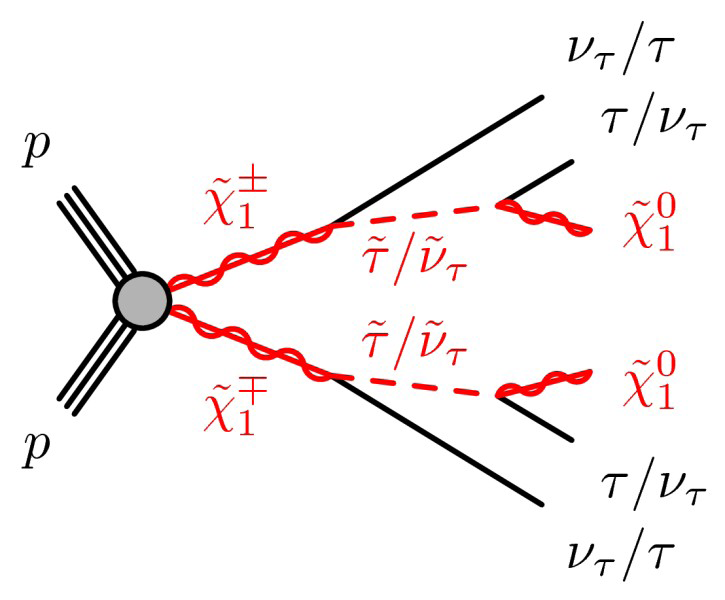
\includegraphics[width=0.3\textwidth]{Introductionfigs/DiChargino.png}
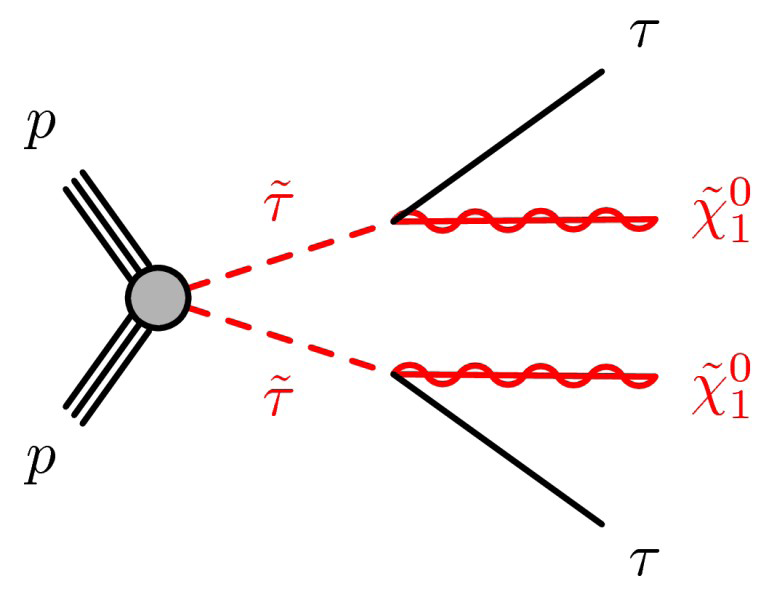
\includegraphics[width=0.3\textwidth]{Introductionfigs/DiSTau.png}
\caption{Schematic production of double tau from chargino pair and stau pair.}
\label{fig:Productions}
\end{figure}

The tau leptons can decay to electron or muon in 35\% of the cases (17.5\% for each lepton) 
or can decay via hadrons in 65\% of the cases. Since there are two leptons in the final state, then the probability of having 
two hadronic tau, \tauTau is 42\% and Lepton-\Tau is 46\%. We will see that having less background in \tauTau channel, makes it more powerful
in the final exclusion, although the branching ratio is a little lower.

The search variable which is used to distinguish between the signal and background is the stransverse mass (\mttwo) 
which is the natural extension of the known transverse mass (\mt) to a case 
when two massive particles with equal mass are created in pairs and decay via a chain of jets and leptons to two 
invisible particles. 
In the case of R-Parity conserving SUSY, the Lightest Supersymmetric Particle (LSP) escapes the detection and appears as 
a missing transverse momentum.
The distribution of \mttwo reflects the mass difference between the produced particles and the invisible  particles and is higher for sparticles
compared to the SM particles. Hence, SUSY should appear as an excess in the tail of the \mttwo distribution.
It was shown previously \cite{Chatrchyan:2012jx} that \mttwo is a powerful variable to search for SUSY. 




After introduction in the next section the \mttwo variable is introduced. 





\section{\texorpdfstring{The definition of $\rm {\mttwo}$}{The definition of MT2}}
\label{sect:mt2def}
The $\mttwo$ variable~\cite{Lester:1999tx,Barr:2003rg} is used in this analysis to discriminate between the SUSY signal and the SM backgrounds as proposed in~\cite{Barr:2009wu}. The variable was originally introduced to measure the mass of primary pair-produced particles, decaying eventually to undetected particles (e.g. neutralinos). Assuming the two primary supersymmetric particles undergo the same decay chain with visible and undetectable particles in the final state, the system can be described by the visible mass ($\mvisi$), transverse energy ($\etvisi$), and transverse momentum ($\vptvisi$) of each branch ($i=1,2$), together with the 
missing transverse momentum (\ptvecmiss) which is shared between the two decay chains. The \ptvecmiss is interpreted as the sum of the transverse momenta
of the neutralinos, $\vec{p}_{\rm T}^{\PSGczDo(i)}$.
However, in practice, in decay chains with neutrinos, \ptvecmiss includes contributions from the $\pt$'s of the neutrinos.
% $\pt^{\nu}$'s.

The transverse mass of each branch can be written as 
\begin{linenomath}
\begin{equation}
\label{eq:mtdef}
(\mt^{(i)})^{2}= (\mvisi)^2+m^2_{\PSGczDo}+2(\etvisi\et^{\PSGczDo(i)}-{\vptvisi}.\,{\vec{\pt}^{\PSGczDo(i)}}).
\end{equation}
\end{linenomath}

\noindent Using the correct neutralino mass, this distribution has an endpoint at the mass of the primary particle~\cite{Arnison:1983rp,Banner:1983jy,Affolder:2000bpa,Abazov:2002bu}. 
% similar to the W boson transverse mass used to measure $m_{\rm W}$
%As a generalization of the transverse mass, the $\mttwo$ variable is proposed to overcome the problem of unknown $\pt^{\PSGczDo(i)}$. The kinematic endpoint of $\mttwo$ carries model independent information about the mass difference between the primary and the secondary particles. 
For a given $m_{\PSGczDo}$, the $\mttwo$ variable is defined as
\begin{linenomath}
\begin{equation}
\label{eq:mt2def}
\mttwo(m_{\PSGczDo})= \min_{\vec{p}_{\rm T}^{\PSGczDo(1)}+\vec{p}_{\rm T}^{\PSGczDo(2)}=\ptvecmiss}\,\left[\,\max\,\{ \, \mt^{(1)},\,\mt^{(2)}\,\}\,\right].
\end{equation}
\end{linenomath}

For the correct value of $m_{\PSGczDo}$, the kinematic endpoint of the $\mttwo$ distribution is at the mass of the primary particle, and it shifts accordingly when the assumed $m_{\PSGczDo}$ is lower or higher than the correct value. In this analysis we set
$m_{\PSGczDo}=\mvisi=0$.
The visible part of the decay chain consists of either the two hadronically decaying tau leptons ($\hadtau \hadtau$ channel)
or a combination of a muon or an electron with a $\hadtau$ candidate ($\leptonTau$ channel).

%With our choices of $m_{\PSGczDo}$ and $\mvisi$, the resulting $\mttwo$ 
%in back-to-back events (e.g., QCD di-jets) is close to zero, regardless of the values of $\MPT$ and the $\pt$ of the $\tau$ candidates.
%This is to be contrasted with the case of signal where the taus or leptons are in general not back-to-back 
%due to the presence of two undetected neutralinos.
%the visible system is not back-to-back and  \mttwo has larger values.
%variable is expected to well reject not only events with no genuine $\MPT$ but events with a back-to-back topology ($\mttwo=0$) . 

With  our choices of $m_{\PSGczDo}$ and $\mvisi$, the resulting \mttwo value is close to zero for back-to-back topology of \tauTau or \leptonTau  
events (e.g., Drell-Yan events; QCD di-jets if two jets are misidentified as \Tau objects), regardless of the values of \MPT and the \PT of 
the tau candidates. This is not the case for signal events where the taus or leptons are generally not in back-to-back topology due 
to the presence of two undetected neutralinos.

The distribution of \mttwo reflects the scale of the produced particles and is much higher for heavy sparticles
compared to the lighter SM particles. Hence, SUSY 
could manifest itself
as an excess of events in the high-side tail of the \mttwo distribution.
% It was shown previously \cite{Khachatryan:2014qwa} and \cite{Chatrchyan:2012jx}    
% that \mttwo is a powerful variable to search for SUSY in both leptonic and hadronic final states.

\section{Datasets and MC samples}
\label{sect:dataMC}
To reconstruct the objects, the CMSSW\_5\_3\_7\_patch5 is used for both data and Monte Carlo(MC).
The data used in this analysis corresponds to 18.1 \fbinv in \hadtau\hadtau channel and 19.6 \fbinv in $l\hadtau$ channel of proton-proton collisions in the center of mass energy of $\sqrt{s}$ = 8 TeV 
which was taken in 2012. The datasets used for $e\tau_{had}$, $\mu\tau_{had}$ and $\tau_{had}\tau_{had}$ channels, the run range and the corresponding integrated luminosities are mentioned Table ~\ref{Tab.DataSamples}.
\begin{table}[!Hhtb]

\begin{center}
\small{
\begin{tabular}{|l|c|c|}
\hline
Dataset Name & Run--range & Luminosity(\fbinv) \\
\hline
\multicolumn{3}{|c|}{$e\tau_{had}$ and $\mu\tau_{had}$ channels} \\
\hline
/TauPlusX/Run2012A-22Jan2013-v1/AOD   & 190456--193621 & 0.887\\
/TauPlusX/Run2012B-22Jan2013-v1/AOD   & 193833--196531 & 4.446\\
/TauPlusX/Run2012C-22Jan2013-v1/AOD   & 198022--203742 & 7.153\\
/TauPlusX/Run2012D-22Jan2013-v1/AOD   & 203777--208686 & 7.318\\
\hline
\multicolumn{3}{|c|}{$\tau_{had}\tau_{had}$ channel} \\
\hline
/Tau/Run2012A-22Jan2013-v1/AOD   & 190456--193621 & 0.887 \\
/TauParked/Run2012B-22Jan2013-v1/AOD & 193833--196531 & 4.446 \\
/TauParked/Run2012C-22Jan2013-v1/AOD & 198022--203742 & 7.153 \\
/TauParked/Run2012D-22Jan2013-v1/AOD & 203777--208686 & 7.318 \\
\hline

\end{tabular}
}
\end{center}
\caption{
  List of datasets analysed by different channels.
}
\label{Tab.DataSamples}
\end{table}

For data the golden JSON file,{\small Cert\_190456-208686\_8TeV\_22Jan2013ReReco\_Collisions12\_JSON.txt} is used and it can be found in Table.~\ref{Tab.Triggers} the list of trigger paths which is used for this analysis data. 
\begin{table}[!Hhtb]
\small{
\begin{center}
\begin{tabular}{|l|c|c|}
\hline
HLT Path   & L1 Seed  & Luminosity(\fbinv) \\
\hline
\multicolumn{3}{|c|}{$e\tau_{had}$ channel} \\
\hline
Ele20\_CaloIdVT\_CaloIsoRhoT\_TrkIdT\_TrkIsoT\_LooseIsoPFTau20 & $^{1}$                 &  $0.7$    \\
Ele22\_eta2p1\_WP90Rho\_LooseIsoPFTau20                        & $^{2}$                 & $18.7$    \\   
\hline
\multicolumn{3}{|c|}{$mu\tau_{had}$ channel} \\
\hline
IsoMu18\_eta2p1\_LooseIsoPFTau20                               &    SingleMu16er        &  $0.7$  \\
IsoMu17\_eta2p1\_LooseIsoPFTau20                               &    SingleMu14er        & $18.7$  \\
\hline
\multicolumn{3}{|c|}{$\tau_{had}\tau_{had}$ channel} \\
\hline
DoubleMediumIsoPFTau35\_Trk5\_eta2p1                          &  $^{3}$                       & $3.9$ \\
DoubleMediumIsoPFTau35\_Trk1\_eta2p1                          &  $^{3}$                       & $14.2$ \\
\hline
\end{tabular}
\end{center}
$^{1}$ SingleIsoEG18er or SingleEG20 \\
$^{2}$ SingleIsoEG18er or SingleIsoEG20er or SingleEG22 \\
$^{3}$ L1\_DoubleTauJet44er or L1\_DoubleJetC64 \\
}
\caption{
  Trigger paths used by $e\tau_{had}$, $\mu\tau_{had}$ and $\tau_{had}\tau_{had}$ channels
  for $2012$ data. All the paths given in the table remained unprescaled during the whole and $2012$ data--taking period.
}
\label{Tab.Triggers}
\end{table}
MC samples are used for different standard model backgrounds and signals. These samples are officially generated and reconstructed by the CMS collaboration. The full list of the MC samples and their cross sections are given in Table ~\ref{Tab.MCSamples}. For most of the samples the most accurate calculation of the cross sections available in the literature (usually NLO and NNLO) are used. 
\begin{table}[!Hhtb]
\begin{center}
\small{
\begin{tabular}{|l|c|}
\hline
\multicolumn{2}{|c|}{MC samples } \\
\hline
%Dataset Description                &   
Dataset Name                                            & Cross-Section (pb)    \\
\hline
\multicolumn{2}{|c|}{QCD used in $e/\mu\tau_{had}$ channels }\\
\hline
%QCD BCtoE                        &    
/QCD\_Pt\_20...inf\_BCtoE\_TuneZ2star\_8TeV\_pythia6                & Ref. ~\cite{Prep}\\ 
%QCD EM\_Enriched                 &    
%/QCD\_Pt\_20...inf\_EMEnriched\_TuneZ2star\_8TeV\_pythia6           & Ref. ~\cite{Prep}\\
%QCD Mu\_Enriched                 &
/QCD\_Pt-15...inf\_MuEnrichedPt5\_TuneZ2star\_8TeV\_pythia6         & Ref. ~\cite{Prep}\\
%$\gamma$+jets                       &
/GJets\_HT-40...inf\_8TeV-madgraph                                  & Ref. ~\cite{Prep}\\
\hline
\multicolumn{2}{|c|}{QCD used in $\tau_{had}\tau_{had}$ channel }\\
\hline
%QCD                                &   
/QCD\_HT-100...inf\_TuneZ2star\_8TeV-madgraph-pythia6            &\\
\hline

\multicolumn{2}{|c|}{Top }\\
\hline
%Single top (tW)                    &   
/T\_tW-channel-DR\_TuneZ2star\_8TeV-powheg-tauola       & $22.4$                \\
%Single anti-top ($\bar{\rm t}$W)   &   
/Tbar\_tW-channel-DR\_TuneZ2star\_8TeV-powheg-tauola    & $22.4$\\
%Single top ($s$-channel)           &   
/T\_s-channel\_TuneZ2star\_8TeV-powheg-tauola           & $3.8$\\%3.79
%Single anti-top ($s$-channel)      &   
/Tbar\_s-channel\_TuneZ2star\_8TeV-powheg-tauola        & $1.8$\\%1.76
%Single top ($t$-channel)           &   
/T\_t-channel\_TuneZ2star\_8TeV-powheg-tauola           & $56.4$\\
%Single anti-top ($t$-channel)      &   
/Tbar\_t-channel\_TuneZ2star\_8TeV-powheg-tauola        & $30.7$\\

%$\ttbar$                           & 
/TTJets\_MassiveBinDECAYTTJets\_TuneZ2star\_8TeV  &  $245.8$       \\
-madgraph-tauola                                        &               \\
%$\ttbar$+$\gamma$+ jets              &
/TTGJets\_8TeV-madgraph                                  &  $2.2$              \\%2.166
%$\ttbar$\,+\,Higgs + jets              &
/TTH\_Inclusive\_M-125\_8TeV\_pythia6                    &  $0.1$               \\
%$\ttbar$\,+\,W + jets                  &
/TTWJets\_8TeV-madgraph                                  &  $0.2$              \\
%$\ttbar$\,+\,Z + jets                  &
/TTZJets\_8TeV-madgraph                                  &  $0.2$                \\
%$\ttbar$\,+\,WW + jets                 &
/TTWWJets\_8TeV-madgraph                                 &  $0.002$\\%$2\times 10^{-3}$                \\

\hline
\multicolumn{2}{|c|}{$ZX$ }\\
\hline
%Z $\rightarrow \ell\ell$                 &
/DYJetsToLL\_M-10To50filter\_8TeV-madgraph-tarball      &   $876.8$               \\
%Z $\rightarrow \ell\ell$                &  
/DYJetsToLL\_M-50\_TuneZ2Star\_8TeV-madgraph-tarball    &   $3503.7$               \\
%Z + 1 jet                           &   
/DY1JetsToLL\_M-50\_TuneZ2Star\_8TeV-madgraph           &   $666.3$               \\
%Z + 2 jets                          &   
/DY2JetsToLL\_M-50\_TuneZ2Star\_8TeV-madgraph           &   $215.0$               \\
%Z + 3 jets                          &   
/DY3JetsToLL\_M-50\_TuneZ2Star\_8TeV-madgraph           &   $60.7$               \\
%Z + 4 jets                          &   
/DY4JetsToLL\_M-50\_TuneZ2Star\_8TeV-madgraph           &   $27.3$               \\
%WZ                                 &   
/WZJetsTo3LNu\_TuneZ2\_8TeV-madgraph-tauola             &  $1.1$                \\
%WZ                                 &   
/WZJetsTo2L2Q\_TuneZ2star\_8TeV-madgraph-tauola         &  $2.2$                \\
%ZZ                                 &   
/ZZJetsTo4L\_TuneZ2star\_8TeV-madgraph-tauola           &  $0.2$                \\
%ZZ                                 &   
/ZZJetsTo2L2Nu\_TuneZ2star\_8TeV-madgraph-tauola        &  $0.7$                \\
%ZZ                                 &   
/ZZJetsTo2L2Q\_TuneZ2star\_8TeV-madgraph-tauola         &  $2.5$                \\
\hline
\multicolumn{2}{|c|}{W}\\
\hline

%W + jets                           &   
/WJetsToLNu\_TuneZ2Star\_8TeV-madgraph-tarball          &  $36257.2$              \\
%W + 1 jet                           &   
/W2JetsToLNu\_TuneZ2Star\_8TeV-madgraph-tarball         &  $6381.2$               \\
%W + 2 jets                          &   
/W2JetsToLNu\_TuneZ2Star\_8TeV-madgraph-tarball         &  $2039.8$               \\
%W + 3 jets                          &   
/W3JetsToLNu\_TuneZ2Star\_8TeV-madgraph-tarball         &  $612.5$               \\
%W + 4 jets                          &   
/W4JetsToLNu\_TuneZ2Star\_8TeV-madgraph-tarball         &  $251.0$                \\
\hline
\multicolumn{2}{|c|}{WW}\\
\hline
%WW                                 &   
/WWJetsTo2L2Nu\_TuneZ2star\_8TeV-madgraph-tauola        &  $5.8$                \\

\hline
\multicolumn{2}{|c|}{Higgs}\\
\hline
%WW                                 &   
/GluGluToHToTauTau\_M-125\_8TeV-powheg-pythia6          &  $1.2$                \\
/VBF\_HToTauTau\_M-125\_8TeV-powheg-pythia6             &  $0.1$                \\
/WH\_ZH\_TTH\_HToTauTau\_M-125\_8TeV-pythia6-tauola     &  $0.08$\\
%$$8\times10^{-2}$                \\

\hline

\end{tabular}
}
\end{center}

\caption{List of MC samples used as backgrounds produced in /Summer12-DR53X-PU\_S10\_START53\_*/AODSIM scenario.}
\label{Tab.MCSamples}
\end{table}

The investigated SUSY signal in this analysis is {\small $pp \rightarrow \chip \chim \rightarrow \tau^+ \tau^- \MET$} called {\small "TChipChimSlepSnu"} produced with \PYTHIA $6.0$ at the level of LHE. \TAUOLA is used to decay precisely the produced $\tau$'s, then the generated events are
passed through the CMS official Fast-Sim process.


\section{Physics Object Definition}
\label{sect:objdef}
To define the physics objects of the analysis, we follow the recommendations and selections of another CMS analysis which search for Higgs bosons decaying to $\tau$ pairs \cite{CMS_AN_2013-188}. Due to the very similar final states, it is well motivated to avoid duplication of the efforts to define and optimize the object selections. For the completeness of the note, the object selections are reviewed shortly here. More detail can be found in \cite{CMS_AN_2013-188} and \cite{HiggsTauTautwiki}

\subsection{Electron}
Electron identification is based on a MVA (Boosted Decision Tree) method ~\cite{Hocker:2007ht} which also cleans the colletion of electron from jet\,$\rightarrow e$  fakes. The training process takes advantage of two bins of $\pt$ and three bins of $\eta$, running over a sample of $Z \rightarrow ee$  events selected in data. Those oppositely charged electrons pair closest to Z-boson peak mass is taken as "signal" and the other electron candidates as "background". The training input variables are described in ~\cite{CMS_AN_2013-188}. Different discriminators are trained on electrons passing the criteria of single electron trigger and also on non triggered electrons. In this analysis the latter case is chosen.   
Depending on the BDT output, a loose and tight working point of \textit{ElIDMVANoTrig} algorithm can be defined. The citeria in different bins of $\pt$ and $\eta$ are given in Table ~\ref{Tab.electronMVAIDwp}.

\begin{table}[!h]
\begin{center}
\begin{tabular}{|l|l|c|c|}
\hline\hline
\multicolumn{2}{|c|}{Kinematic range}                & Loose & Tight \\
\hline\hline
\multirow{3}{*}{$\pt < 20$~\GeV} & $\vert \eta \vert < 0.8$         & 0.925 & 0.925 \\
                  & $0.8 < \vert \eta \vert < 1.479$ & 0.915 & 0.915 \\
                  & $\vert \eta \vert > 1.479$       & 0.965 & 0.965 \\\hline
\multirow{3}{*}{$\pt > 20$~\GeV} & $\vert \eta \vert < 0.8$         & 0.905 & 0.925 \\
                  & $0.8 < \vert \eta \vert < 1.479$ & 0.955 & 0.975 \\
                  & $\vert \eta \vert > 1.479$       & 0.975 & 0.985 \\
\hline\hline
\end{tabular}
\end{center}
\caption{
  Discriminator thresholds for the Loose and Tight MVA electron identification working--points respectively.
}
\label{Tab.electronMVAIDwp}
\end{table}     

To reject those electrons which is coming from photon conversions, it is required that the electron touches all layers of Pixel detector. Furthermore if there is an oppositely charged track near electron which is fitted to a common vertex inside of tracker volume that electron is rejected.  
\subsection{Muon}
Muons are required to be reconstructed by the Tracker or the Global muon reconstruction algorithm and to be identified as 
muons by tight particle flow algorithm.

The particle flow algorithm identifies  muons by applying several criteria.

$\bullet$ The number of pixel hit(s) associated to muon track\,$\geq $\,1

$\bullet$ Number of tracker layers with hits should be $\geq $\,6

$\bullet$ The number of hits in muon system $\geq $\,1

$\bullet$ Tracker track matched with at least one muon segment (in any station)

$\bullet$ $\chi ^{2}/{\rm NDF} $ for the global track fit\,$< $\,10 ,

$\bullet$ Impact parameter constrains between the muon track and the selected primary vertex 
 $d_{z} < $\,0.5 cm and $d_{0} <$\,0.2 cm.

\subsection{Muon and electron isolation}

In order to reduce the background contributions from QCD multi–jet events, electrons and
muons are required to be isolated. The isolation is computed as the $\pt$ sum of charged particles (including charged hadrons, 
electrons and muons), neutral hadrons plus photons reconstructed by the PF algorithm within a cone of size
$\Delta R_{\rm iso}$ = 0.4 (0.3) around the direction of the muon (electron). 
In the innermost region
(``veto cone'') neutral
hadrons and photons  are excluded from the computation of the isolation $\pt$ sum in order to prevent energy deposits in the electromagnetic and hadronic calorimeters. Charged particles close to the direction of electrons  are excluded too in order to avoid tracks due to conversions of photons emitted by Bremsstrahlung processes to spoil the isolation.

For the lepton isolation the photon and neutral hadron candidates are required to have a transverse energy of $\pt>0.5\,\GeV$. This reduces pile-up effects. The correction of pile-up to isolation is done by applying $\Delta\beta$ corrections.
\begin{linenomath}
\begin{equation}
\label{eq:muonisolation1}
I_{e/ \mu}\,=\,\Sigma\, \pt^{\rm charged }(\Delta z <2\,mm)+max(\pt^{\rm photon}+\pt^{h0 }-\Delta \beta,0),
\end{equation}
\end{linenomath}
The $\Delta\beta$ corrections are computed by summing the transverse momenta of charged particles
that have longitudinal impact parameters $\Delta z > 2$ mm with respect to the lepton production
vertex and scaling the sum by a factor 0.5:
\begin{linenomath}
\begin{equation}
\label{eq:muonisolation2}
\Delta\beta\,=\,0.5\, \Sigma \pt^{\rm charged }(\Delta z > 2mm).
\end{equation}
\end{linenomath}

\subsection{\texorpdfstring{Hadronic $\tau$}{Hadronic tau}} 
\label{sec:hadTau}
The "Hadron plus Strip" (HPS) algorithm~\cite{2012JInst...7.1001C} is employed to reconstruct the hadronic decays of $\tau$ leptons with the jet constituents as input. The algorithm is seeded by PF jets reconstructed using the anti-$k_{\rm T}$ procedure with a distance parameter of $R=0.5$. To discriminate against quark and gluon jets, jets with extra particles not compatible with the hadronic $\tau$ decays are rejected. Additional criteria are used to suppress the contributions from electrons and muons in the hadronic $\tau$ ($\hadtau$) collection.

Based on the expected particles in the final state of the hadronic $\tau$ decay, different combinations of charged hadrons and $\pi^0$ candidates are considered. The $\pi^0 (\to\gamma\gamma)$ candidates are reconstructed using PF photons with $\pt>2.5\,\GeV$, falling into $\eta-\phi$ "strips" with specific size~\cite{CMS_AN_2013-171}. While a \textbf{single charged hadron} is an indication of $\tau^{\pm}\to\pi^{\pm}\nu_{\tau}$, a combination of \textbf{three charged hadrons} fulfilling a set of requirements are considered as the process of $\tau^{\pm}\to a_1^{\pm}\nu_{\tau}\to\pi^{\pm}\pi^{\mp}\pi^{\pm}\nu_{\tau}$. \textbf{One charged hadron plus two Strips} with a dedicated selection is assigned to $\tau^{\pm}\to a_1^{\pm}\nu_{\tau}\to\pi^{\pm}\pi^{0}\pi^{0}\nu_{\tau}$ decays. Finally the signature of  $\tau^{\pm}\to\rho^{\pm}\nu_{\tau}\to\pi^{\pm}\pi^{0}\nu_{\tau}$ decay is searched for in \textbf{one charged hadron plus one Strip} combinations. All charged hadrons and strips in the $\tau$ decay mode reconstruction must be within a narrow cone around the jet axis where the cone size depends on the $\tau$ jet $\pt$. Details on specific selections for each category as well as the $\pt$ dependence of the cone size can be found in Ref.~\cite{CMS_AN_2013-171}

The isolation variable is defined as the sum of the $\pt$ of charged hadrons and the $\et$ of photons within a cone of $\Delta R = 0.5$ around the $\hadtau$ axis. Particles used to reconstruct the $\hadtau$ candidate are excluded. The contribution of pile-up to the $\Tau$ isolation is accounted for by applying the so-called $\Delta\beta$ corrections. The selection criteria for charged hadrons in the isolation sum together with the pile-up subtraction procedure can be found in Ref.~\cite{CMS_AN_2013-171}. The Loose, Medium and Tight working points of {\it CombinedIsoDBSumPtCorr3Hits} algorithm correspond to isolation variables less than 2.0, 1.0 and 0.8\,$\GeV$, respectively.

The $\hadtau$ candidates are vetoed if signals exist in the muon system close to the $\hadtau$ direction. Loose, Medium and Tight working points are provided, corresponding to different $\hadtau$ identification efficiencies and $\mu\to\hadtau$ fake rates~\cite{CMS_AN_2013-171}. To discriminate against electrons i.e., rejecting $e\to\hadtau$ fakes, a multivariate discriminator is trained for which the Loose, Medium, Tight and very-Tight working points are defined based on the outputs of 16 different BDT's. Each BDT is associated to a category of $\hadtau$ candidates where the classification of $\hadtau$'s is performed according to their kinematics and decay mode as well as their closeness to a GSF electron. The working points are optimized to achieve the lowest $e\to\tau$ rate possible with a given $\hadtau$ identification efficiency~\cite{CMS_AN_2012-417}.

%Tau leptons from Higgs boson decays are expected to be isolated in the detector, while leptons from heavy-flavor (c and b) decays and decays in flight are expected to be found inside jets. A measure of isolation is used to discriminate the signal from the QCD multijet background, based on the charged hadrons, photons, and neutral hadrons falling within a cone around the lepton momentum direction.
%Electron, muon, and tau lepton isolation are estimated as
%\begin{equation}\begin{aligned}
%I_{\Pe,\Pgm} &=  \sum_{\rm charged}  \pt + \text{max}\left( 0, \sum_{\rm neutral}  \pt
%                                        +  \sum_{\gamma} {\pt} - 0.5 \sum_{\rm charged, pileup} \pt  \right ), \\
%I_{\Tau} &=  \sum_{\rm charged}  \pt + \text{max}\left( 0, \sum_{\gamma} {\pt} - 0.46 \sum_{\rm charged, pileup} \pt  \right ),
%\label{eq:reconstruction_isolation}
%\end{aligned}\end{equation}
%where $\sum_\text{charged}\pt$ is the scalar sum of the transverse momenta of the charged hadrons, electrons, and muons from the primary vertex located in a cone centered around the lepton direction of size $\Delta R = \sqrt{(\Delta\eta)^2+(\Delta\phi)^2}$ of 0.4 for electrons and muons and 0.5 for tau leptons.
%The sums $\sum_\text{neutral}\pt$ and $\sum_{\gamma} \pt$ represent the same quantities for neutral hadrons and photons, respectively. In the case of electrons and muons the innermost region is excluded
%to avoid the footprint in the calorimeter of the lepton itself from entering the sum.
%Charged particles close to the direction of the electrons are excluded as well, to prevent tracks originating from the conversion of photons emitted by the bremsstrahlung process from spoiling the isolation. In the case of \Tau, the particles used in the reconstruction of the lepton are excluded. The contribution of pileup photons and neutral hadrons
%is estimated from the scalar sum of the transverse momenta of charged hadrons from pileup vertices in the isolation cone $\sum_\text{charged, pileup}$. This sum is multiplied by a factor of 0.5 that approximately corresponds to the ratio of neutral-to-charged hadron production in the hadronization process of inelastic $\Pp\Pp$ collisions. In the case of \Tau, a value of 0.46 is used, as the neutral hadron contribution is not used in the computation of $I_{\tauh}$. An $\eta$, \pt, and lepton-flavor dependent threshold on the isolation variable is applied.


\subsection{Jet and MET reconstruction}
\label{sec:jetmet}
Particle flow algorithm is used to reconstruct jets and \ETmiss. The medium working point of the Combined Secondary Vertex algorithm is used to tag bjets.

The minimum $\Delta\phi$ between \ETmiss and jets, hereafter referred to as \mindphifour, is used in this analysis to suppress QCD events. To calculate \mindphifour, all the pf-jets in $|\eta|<5.0$ region and with $\pt>40\GeV$ are used without applying any extra identification. $\mindphifour > 1.0$ is found useful for this analysis.


%\section{Search Strategy}
\label{sect:search}
The \mttwo distribution \ref{fig:MT2}
\begin{figure}[!htb]
\centering
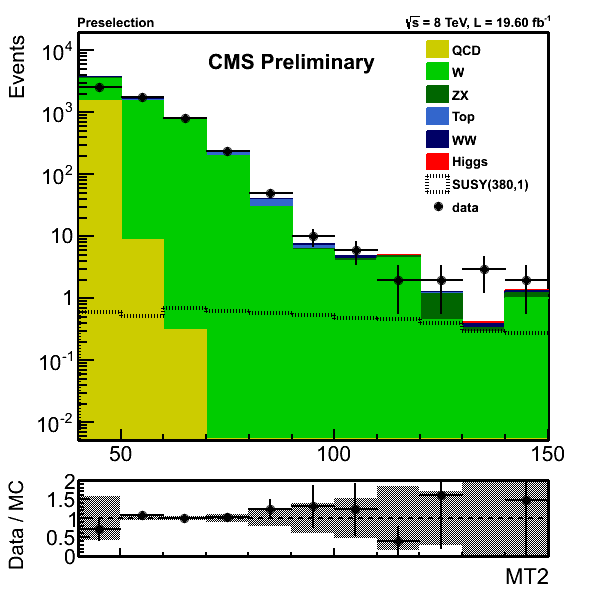
\includegraphics[width=0.49\textwidth]{figs/MT2.png}
\caption{\mttwo distribution after applying the full selection cuts.}
\label{fig:MT2}
\end{figure}
is used as a variable to search for SUSY.
To increase the power of the analysis, a multibinning approach is used.
We select 4 bins in \mttwo with the following edges 125, 150, 200, 250 and infinity.
Every \mttwo bin is devided to two bins with number of the reconstructed top quarks equal to 0 or greater than 0.
There will be 8 bins in the analysis. In this round of analysis, we try to emphasize the complementary role of this anaysis
for the common cut and count hadronic search for the direct stop production. Since this analysis, does not use the MET explicitly, 
it is more sensetive to the small mass differences between stop and LSP.
\section{Backgrounds}
\label{sect:bkg}
In this section, data driven methods are proposed and applied to estimate the contribution of the main background processes. 
Most of the methods are similar to what were used in the \mttwo analysis \cite{MT2_2011} with some minor changes which are explained
here.


\section{Event Selection}
\subsection{Search Strategy}
\label{sect:cuts}
In this analysis, two leptons are created with two missing particles, so \mttwo can be a good discriminator to separate signal 
from the SM backgrounds that leptons are produced from W or Z boson. When the mass difference between the chargino and neutralino 
is sufficiently large, \mttwo can exceed 80 GeV which is the maximum of the \mt of a lepton which comes from the decay of a W boson.
When the mass difference is not sufficiently large, \mttwo of the signal events is below 80 GeV and the signal is buried under the W+jets
backgrounds. In such conditions, $\Sigma\,\mt$ which is defined as $\mt_{,\ell1} + \mt_{,\ell2}$ can be useful to distinguish between the signal and 
SM backgrounds.
To optimize the cuts, two signal points are selected, one with a high mass difference ($m_{\chipm}$ = 380\,\GeV and $m_{\chiz}$ = 1\,\GeV) and
another one with a low mass difference ($m_{\chipm}$ = 180 GeV and $m_{\chiz}$ = 60 GeV). An optimized cut should minimize the signal strength, 
which is the ratio of the measured upper limit on the cross section and the theoretical signal cross section. The details of the statistical 
method can be found in section \ref{sect:stat}.


\section{\texorpdfstring{Event selection for the \tauTau channel}{Event selection for the tau-tau channel}}
\label{sect:tauTauCuts}
In this channel data of proton-proton collisions,  corresponding to an integrated luminosity of 18.1 $\mathrm{fb}^{-1}$, are used.
The events are first selected with a trigger \cite{Chatrchyan:2011nv} that requires the presence of
two \Tau candidates with \PT $>$ 35\GeV and $|\eta|<$ 2.1, which pass loose identification and isolation criteria.

Offline, %the measure of isolation of the two \Tau candidates must be less than 1.5\GeV (medium working point
%of the $\tau$ isolation discriminator \cite{Khachatryan:2015dfa}), 
the two \Tau candidates must pass the tight $\tau$ isolation discriminator,
\PT $>$ 45\GeV and $|\eta|<$ 2.1, and have opposite electric charge (OS).
In events with more than one \tauTau pair, we only consider the pair with the most isolated \Tau objects. 

Events with extra isolated electrons or muons of \PT $>$ 10\GeV and $|\eta| <$ 2.4 
are rejected to suppress %the contribution of the associatiated production of \Z with vector bosons.
backgrounds from diboson decays.
Inspired from the MC studies, to reduce the contribution of the \Z$ \rightarrow$ \tauTau backgrounds, events are  rejected where the visible
di-\Tau invariant mass is between 55 and 85\GeV (\Z boson veto).  
Furthermore, contributions from low-mass DY and QCD multijet production are 
reduced by requiring the invariant mass to be greater than 15\GeV.
Moreover, to further reduce \Z $\rightarrow$ \tauTau and QCD multijet events, %the loose requirements 
\MPT $>$ 30\GeV and \mttwo $>$ 40\GeV are also required.
The minimum angle \deltaphi in the transverse plane between the \ptvecmiss and any of the \Tau and jets, 
including b-tagged jets, must be greater than 1.0 radians. 
This requirement reduces backgrounds from QCD multijet events and \wjets events.

After applying the preselection described above,
additional requirements are introduced to define two search regions.
The first search region (\binone) targets models with large mass difference ($\Delta m$) 
between charginos and neutralinos.
In this case, the \mttwo signal distribution can have a long tail beyond the 
distribution of SM backgrounds.
The second search region (\bintwo) is dedicated to models with small values of $\Delta m$.
In this case, the sum of the two transverse mass values, \SumMT = $\mt(\Tau^1,\ptvecmiss) + \mt(\Tau^2,\ptvecmiss)$, 
provides additional discrimination between signal and SM background processes.

The two signal regions (SR) are defined as:
\begin{itemize}
\item {\bf \binone}: \mttwo $>$ 90\GeV,
\item {\bf \bintwo}:  \mttwo $<$ 90\GeV, \SumMT $>$ 250\GeV, and b-tagged jets are vetoed.
\end{itemize}
The veto on b-tagged jets in SR2 reduces the
\ttbar events, which
are expected in  the low-\mttwo region. Table \ref{Tab.Cuts} summarizes the selection requirements for different signal regions.
\begin{table}[!htb]
\begin{center}
\caption{Definition of signal regions.}
\begin{tabular}{|c|c|c|}
\hline
               & \tauTau & \tauTau               \\
   \leptonTau  & \binone & \bintwo               \\\hline\hline
 OS \leptonTau & \multicolumn{2}{c|}{OS \tauTau}  \\\hline
\multicolumn{3}{|c|}{Extra lepton veto}          \\\hline
\multicolumn{3}{|c|}{Invariant mass of \leptonTau or \tauTau $>$ 15\GeV}\\\hline
\multicolumn{3}{|c|}{\Z boson mass veto}              \\\hline
\multicolumn{3}{|c|}{\MPT $>$ 30\GeV}            \\\hline
\multicolumn{3}{|c|}{\deltaphi $> 1.0 $ radians}         \\\hline
\multicolumn{3}{|c|}{$\mttwo > 40\GeV$}         \\\hline
b-tagged jet veto&  - & b-tagged jet veto  \\\hline
\multicolumn{2}{|c|}{$\mttwo > 90\GeV$} & $\mttwo < 90\GeV$ \\\hline
$\tauMT > 200\GeV$    &  - & $\SumMT > 250\GeV$ \\\hline
\end{tabular}
\label{Tab.Cuts}
\end{center}
\end{table}
%The distributions of $\mttwo$ and $\SumMT$ for data and the SM prediction are shown in Fig.~\ref{fig:comparison} before the application of the final requirements listed above. In the $\SumMT$ distribution, the b-tagged jets are vetoed and \mttwo $<$ 90\GeV is also applied. The SM predictions in Fig.~\ref{fig:comparison} are from simulated events, except for the QCD multijet prediction which is taken from same-sign di-tau data events, after subtracting a small contribution of same-sign non-QCD events estimated from Monte Carlo events. The data and SM predictions are in agreement within the statistical uncertainties.
%The expected distributions for a SUSY signal corresponding to a moderate mass difference $(m_{\chione}=240\GeV,~m_{\PSGczDo}=40\GeV)$ are also shown for illustration purposes.
%\begin{figure}[!htb]
%\centering
%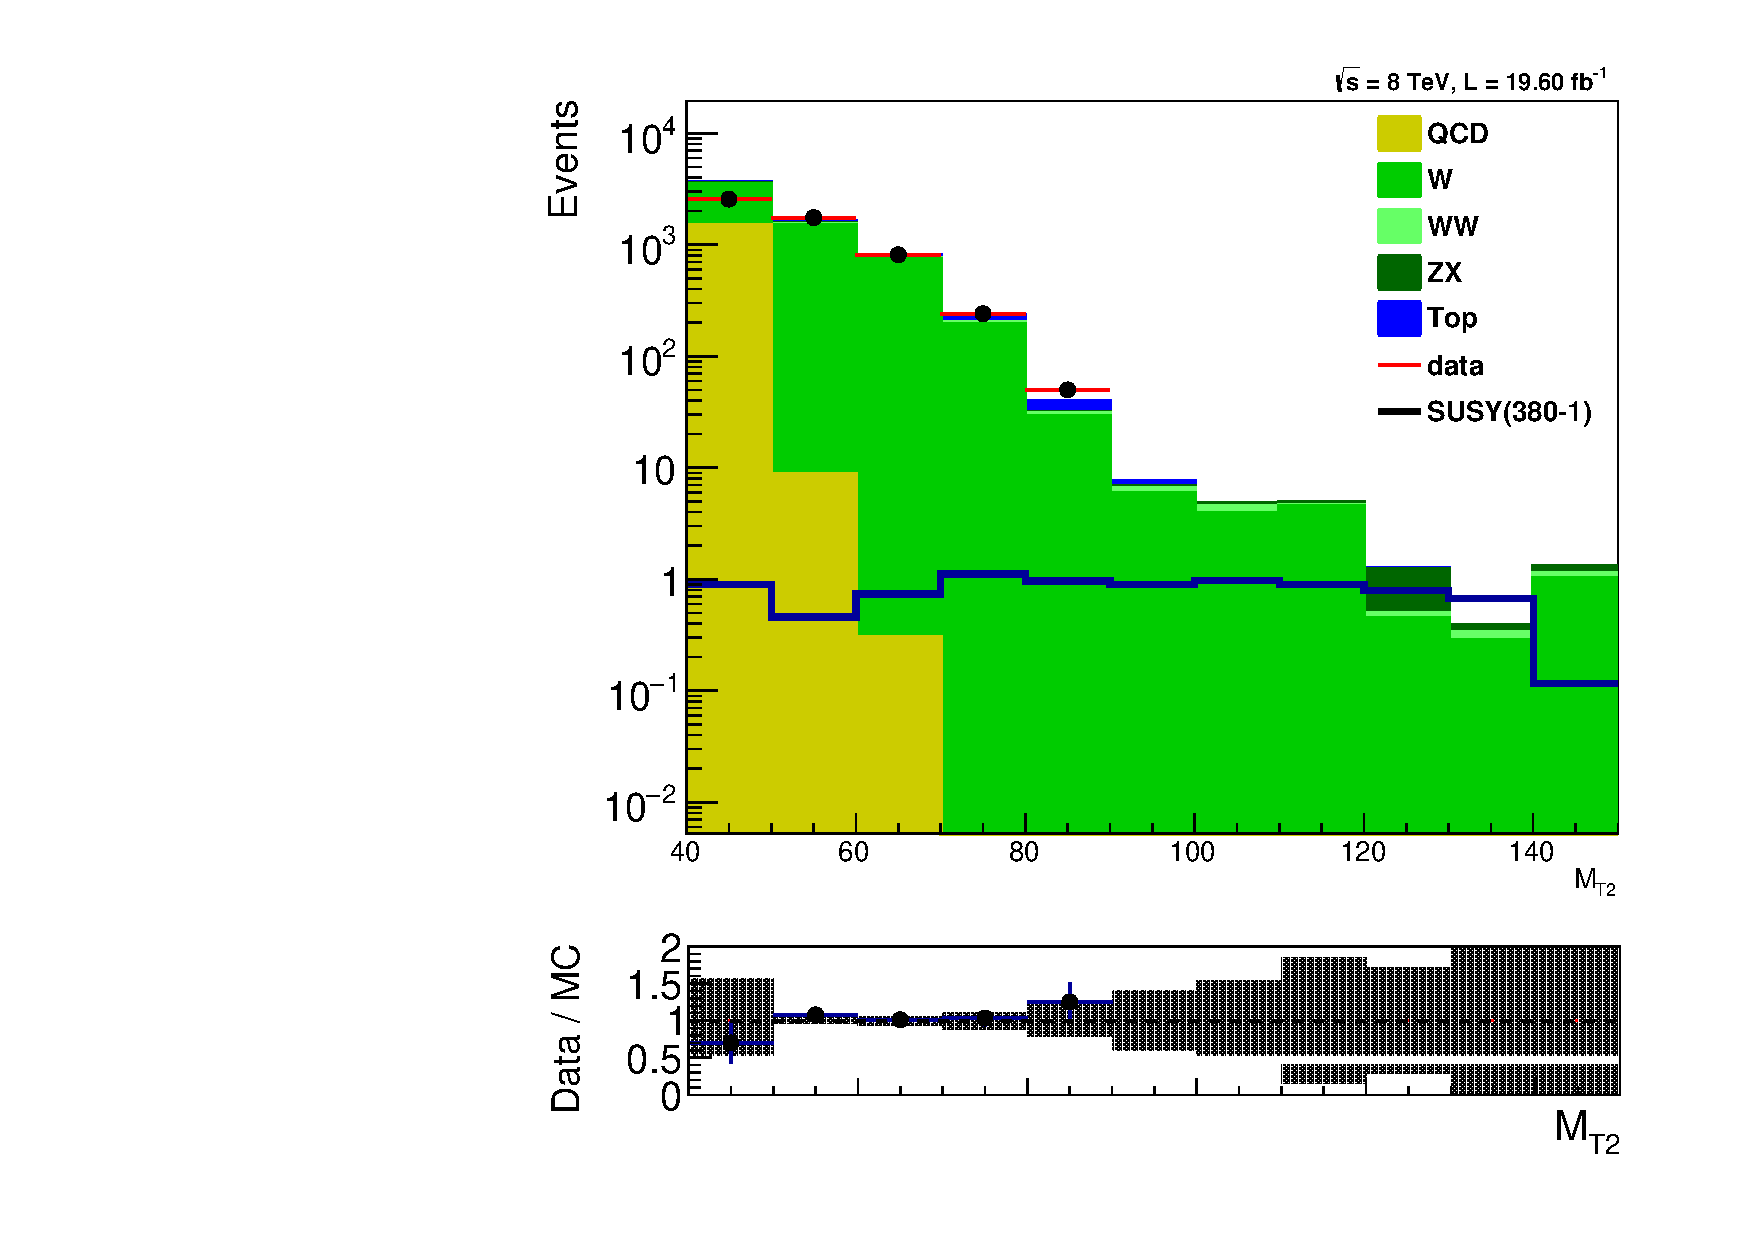
\includegraphics[angle=0,scale=0.375]{TauTauFigs/MT2.pdf}
%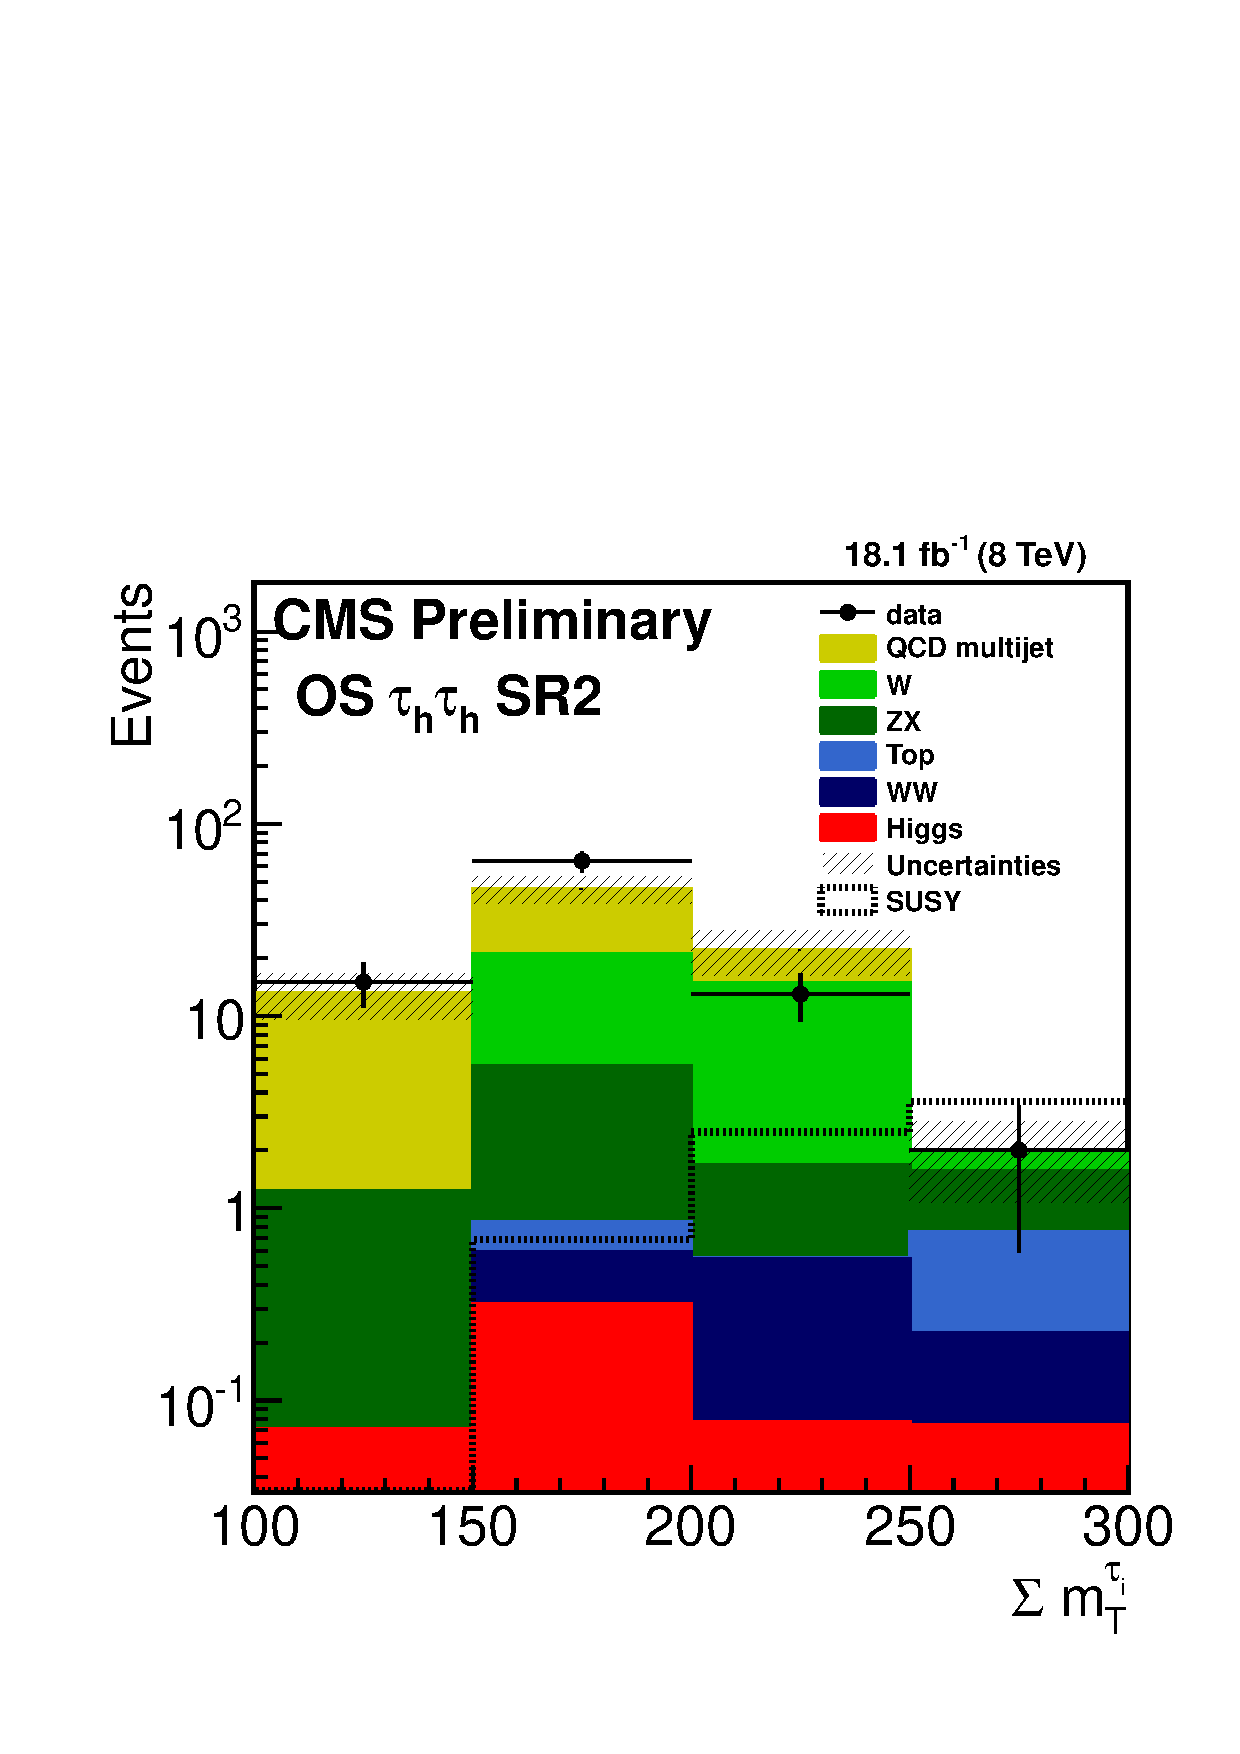
\includegraphics[angle=0,scale=0.375]{TauTauFigs/SumMT.pdf} \\ 
%\caption{The distributions of \mttwo (left) and \SumMT (right) after applying all the selections. 
%The last bins of the histograms correspond to the two signal regions (\binone and \bintwo). The signal distribution is shown for $m_{\chione}=240\GeV,~m_{\PSGczDo}=40\GeV$.}
%\label{fig:comparison}
%\end{figure}

\section{Selection Cuts for muTau Channel}
\label{sect:muTauCuts}

muTau

Saeid



\section{Selection Cuts for eleTau Channel}
\label{sect:eleTauCuts}
In lepton (electron and muon) + hadronic $\tau$ channels, tight isolated $\tau$ objects are selected. To reduce the rate of the fake $\tau$'s orginated from electron and $\mu$, the same cuts on the discriminators against electron and $\mu$ which are used in the Higgs search analysis have been applied. In electron + $\tau$ channel, $\tau$ objects which pass MediumMVA3Rejection against electron and the LooseMuon2RejectionPF discriminator against $\mu$ are selected. In the $\mu + \tau$ channel, the tight working point of the Muon2Rejection is requested and the Loose working point of the discriminator against electron is applied.

 
In electron + $\tau$ channel, each event is requested to have an electron with $p_{T}>20 GeV$ in the $\|\eta\| < 2.1 $ region. A tight cut of $0.1$ on the isolation and $0.1$ on the $dZ$ of the selected electron are also applied.

To supress dilepton and multilepton backgrounds, events with and extra electron or $\mu$ with $p_{T}>10 GeV$ are rejected. For the extra electron, a wider window of $\|\eta\|<2.3$ is scanned and a looser isolation cut of $0.2$ is applied. For the extra $\mu$, a selection similar to the $\mu$ selection in $\mu+\tau$ channel is applied.


After requesting two opposite sign leptons in the events, a loose cut on MET $>30 GeV$ is applied to supress QCD events. As there is no b-quark in the signal, rejecting events with one or more b-tagged jets helps a lot in reducing $t\bar{t}$ and $W+b$ backgrounds.

To reject QCD low mass resonances, the invariant mass of the lepton and the hadronic $\tau$ is requested to be greater than $15\ GeV$. Another cut on the invariant mass of the di-lepton system is applied to remove the peak of the $Z+jets$ events. It has been found that the visible mass of the $Z\to\tau\tau\to\,electron +\,hadronic\,\tau$ moves to $60 \pm 15 GeV$ due to mis-reconstruction of the energy of the hadronic $\tau$ and also the missing energy due to the decay of the $\tau$ to electron. So the window of $45 < Invariant\,Mass < 75$ is cutted away. As the last pre-selection cut, events with $MT2<40 GeV$ are discarded to kill the bulk of the QCD events and get rid of related uncertainities due to mis-reconstruction of the QCD events. As it has mentioned above, the signal events are expected to have high $MT2$ values and are not removed with such a cut.

The cut flow tables for the electron/$\mu$ $\,+\tau$ pre-selections are shown in tables .... and ... respectively. The distribution of the $p_{T}$ of the $\tau$ and $MET$ in the pre-selected events in both channels are shown in FIGS ... . The good agreement between data and MC confirms that the needed correction factors are considrred carefully.

Similar to the di-hadronic $\tau$ channel, first we find the optimized cut on the $MT2$ to supress backgrounds especially $W+jet$ events. As it has been shown in FIG ..., the best value to cut on, similar to the $\tau\tau$ channel is $MT2 > 90 GeV$ for both $e/\mu+\tau$ channels. Such a high cut on the $MT2$ increases the sensitivity of the study to signal events with high $\Delta M_{\chi^{\pm}lsp}$ values. We then investigate the shape of different variables for signal and backgrounds and try to find the most optimized cut to have the best exclusion. The most sensitive variable for both channels are found to be the $\tau$ transverse mass. As it has been shown in FIG ..., the best cut value for the high mass difference signal is $\tau M_{T} > 200 GeV$. You can find the composition of the backgrounds and number of remaining signals for bothe channels in tables ... and ... respectively.

Opposite to the $\tau\tau$ channel, the events with $MT2<90 GeV$ are not useful in electron/$\mu + \tau$ channels because of the contamination of the $W+jets$ events.

\section{Backgrounds}
\label{sect:bkgLepTau}
We separate the backgrounds into two distinct categories.  Those with 
``fake'' \Tau, i.e., events where a quark or gluon jet has been misidentified
as a \Tau, and those without \Tau misidentifications.  
The fake \Tau backgrounds arise mostly from QCD and $W+$ jets events.  The 
other backgrounds are from \ttbar, $Z+$ jets, dibosons, and Higgs decays.
Backgrounds with fake \Tau are estimated with data-driven methods; the 
remaining backgrounds are taken from Monte Carlo.

%In different channels, the contribution of the events with a fake \Tau, namely QCD and $W$jets is estimated using the data. 
%For the prompt \Tau's, from top, $\cPZ$jets, di-boson and higgs we trust 
%the MC, but the important contributions are validated in a signal like region. 
%In this section we will discuss the different background estimation techniques used.
%In continue, estimation of different backgrounds are explained.

\subsection{\texorpdfstring{QCD background estimation in the $\tauTau$ channel}{QCD background estimation in the tau-tau channel}}
%{\bf (I actually could not fully understand from the original text how this is done.
%I rewrote it extensively, according to my understanding, and I took out
%many details that I do  not think are relevant.  In particular, I 
%did not really understand the same-sign business.
%So I what I say about same-sign may be quite wrong).}

Events from QCD can enter the signal regions if two quark or gluon jets are 
misidentified as \Tau, and the rest of the kinematical cuts are also 
satisfied.  Isolation is an important 
discriminant between fake \Tau and prompt \Tau.
Therefore we define control regions in the 
\Tau pair isolation vs. \mttwo or \SumMT 
planes, as shown in Fig.~\ref{fig:ABCDQCD}. We then estimate the QCD background
in the signal regions starting from the event counts in the
control regions under the assumption
that for fake \tauTau the isolation is uncorrelated with \mttwo or \SumMT.
This assumption was checked in the QCD domainated region of data.
%{\bf (Not clear to me what isolation means here, because
%you have two \Tau and therefore two isolations.  Which of the 
%two isolations do you actually use?  This needs to be specified).}

To reduce contamination from prompt \tauTau, in the control regions with at least one loose \Tau, 
the same-sign pairs are selected.  Residual contributions from prompt
\tauTau and $W+$ jets are subtracted off based on Monte Carlo expectations.
In addition, the cut on $\Delta \Phi$
is removed to improve on the statistical power of the method. 
The final estimate of the background
is taken from the control regions extrapolation with corrections
associated with the same-sign requirement and the efficiency of 
the $\Delta \Phi$ requirement for QCD events.


%Due to the large cross section of the QCD multijet events and lack of the statistics, there is a large statistical uncertainty on the 
%yield of the QCD events from MC. On the other hand, 
%The QCD multijet events contribute to the signal selection of the \tauTau channel, when two jets are 
%fakely identified as \Tau's. The fake rate can be different between data and MC, so a data driven method is developed to estimate the 
%contribution of the QCD multijet events. 
%Since the search variable (\mttwo in \binone and \SumMT in \bintwo) and the 
%isolation of the \Tau's are uncorrelated in the QCD events, the ratio of the events selected by the signal cuts over the events 
%with loosely isolated \Tau's should be independent from the search variable, so one can find the ratio in the low \mttwo or \SumMT and 
%multiply it to the number of events in the control region which is defined same as the signal region except the \Tau's are loosely isolated. 
%This would give an estimate of the QCD events in the signal region. In the signal region, loosely isolated  \Tau's 
%($I_{\Tau} <$ 2 \GeV ) 
%are excluded, but in the control region, only the pairs with at least one loosely isolated \Tau are selected. 
%These pairs are requested to be same-sign to suppress the signal contamination. To further increase the statistics 
%in different regions, the cut on the minimum angle in the transverse plane between the \MET and the jets is removed. The final estimation
%is corrected by the efficiency of this cut which is read from data and will be described in continue.

%{\bf It seems to me that this procedure would at the same time estimate 
%the $W+$ jets background with one real \Tau and one fake \Tau. (??)}


\begin{figure}[!Hhtb]
\centering
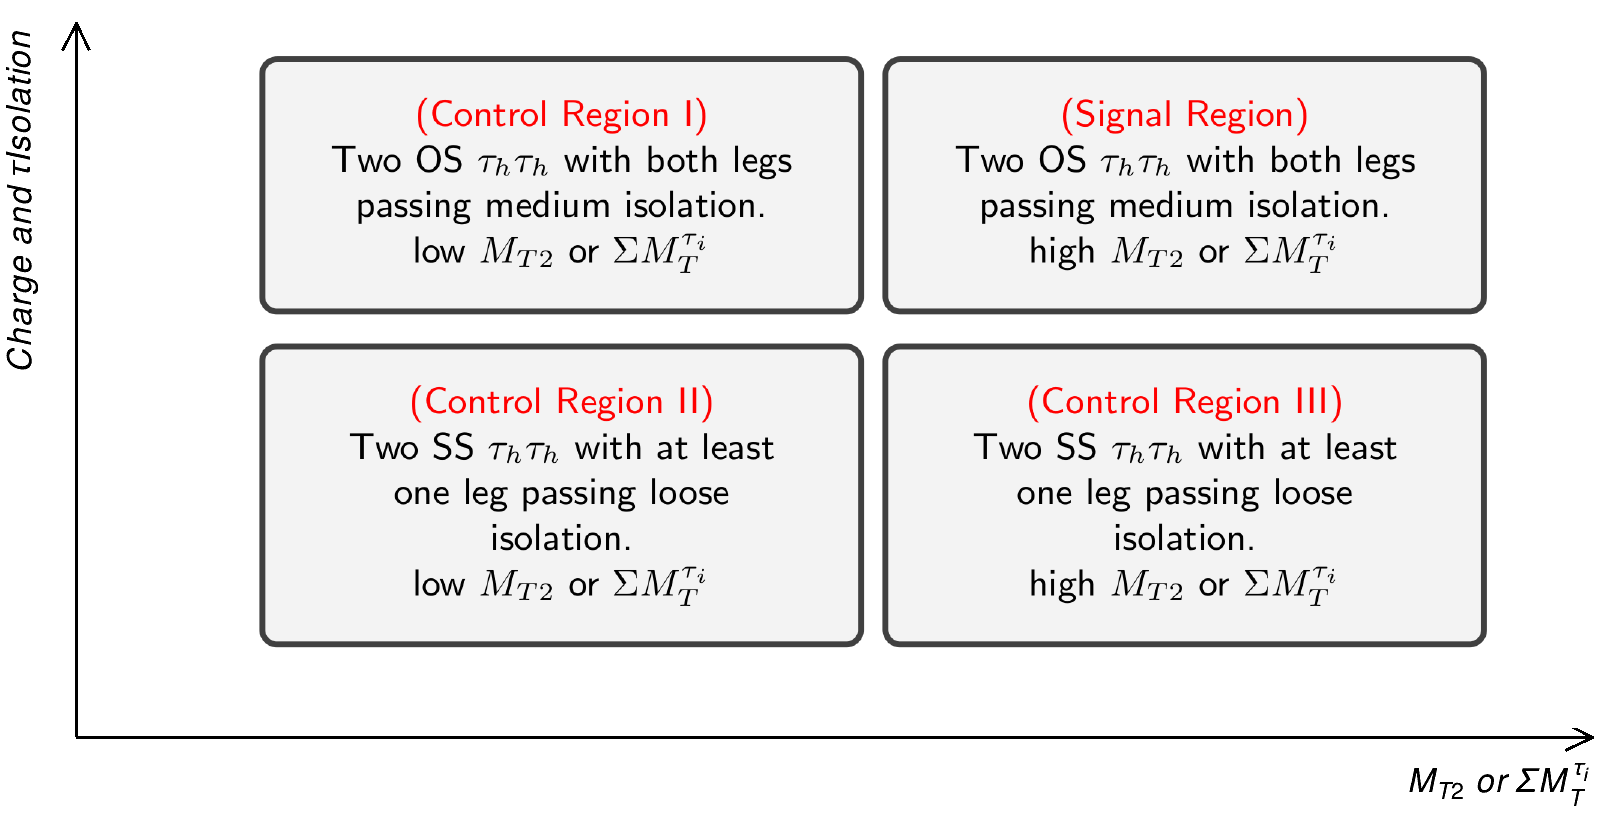
\includegraphics[angle=0,scale=0.30]{Bkg/ABCD.png}
\caption{Schematic description of the regions used to estimate the QCD backgrounds.}
\label{fig:ABCDQCD}
\end{figure}

%Non-QCD events from MC are subtracted from data to find a QCD sample.
%In the low \mttwo or \SumMT of the QCD sample, the ratio of the signal like events over the same-sign loose pairs 
%is found and verified to be flat as a function of the search variable. 
%A horizontal line is fitted to
%This ratio is multiplied to the same-sign loose pairs in high \mttwo or \SumMT and corrected by the efficiency of the 
%cut on the minimum angle between the \MET and the jets, to find the QCD contamination in the signal region. 
%The efficiency of the cut on the minimum angle between the \MET and the jets, is found with the same events as a function of the search variables.
%The value of the efficiency in the last bin in vicinity of the signal region is used to correct the estimation.
%To estimate the systematic uncertainty of the estimated value and take into account the potential correlation between the two values, 
%the method to extract the
%ratio and the efficiency are varied from approximating by a flat line to fitting by a straight line with a floating slope 
%or using the value of the  last bin before the signal region. 
%This is  also a measure  of the correlation between the two variables which are assumed to be uncorrelated. 


\begin{table}[!Hhtb]
\begin{center}
\begin{tabular}{|l|c|}
\hline\hline
 Region      &  Estimation\\
\hline\hline
%SR1      & 0.15 $\pm$ 0.22 $\pm$ 0.13 \\   
SR1      & 0.13 $\pm$ 0.19 $\pm$ 0.10 \\
\hline
%SR2      & 0.82 $\pm$ 0.65 $\pm$ 0.07  \\
SR2      & 1.15 $\pm$ 0.81 $\pm$ 0.25  \\
\hline\hline
\end{tabular}
\caption{The estmated QCD background in the \tauTau channel. The first uncertainty is statistical and systematic of the method, the second is systematic due to correlation assumptions.}
\label{4QCDbg}
\end{center}
\end{table}

Table \ref{4QCDbg} 
summarizes the estimation of the QCD background contribution in the two signal regions after extrapolation from the control regions and 
correcting for the $\Delta \Phi$ efficiency.  
The systematic uncertainties are associated with the uncertainty on the validity 
of the assumption that isolation and \mttwo or \SumMT are not correlated.
%${\bf (I think that this is what you had in the original text,
%but what about the efficiency of the $\Delta \Phi$ requirement and the 
%same-sign vs. opposite-sign business?)}


\subsection{\texorpdfstring{$W$jets background estimation in the $\tauTau$ channel}{Wjets background estimation in the tau-tau channel}}
%{\bf I did not understand this, so I did not try to edit it.  This background has one real \Tau and one fake \Tau.  So according to the claim that fake \Tau cannot be taken from MC, this should be data-driven.  But when I read this it seems like it is done from MC, with complications associated with the fact that you do not have enough statistics in the Monte Carlo.  So, I am confused.}
The contribution of the $W$jets background is taken from simulation. %with a large uncertainty. 
While in \bintwo region the number of simulated $W$jets events is large enough to provide a reliable estimate, in \binone no such events remain after the final requirement of \mttwo $>$ 90 \GeV. Therefore, a valid estimation for the efficiency of this requirement, $\epsilon_{\rm M_{T2}>90}$, is necessary to determine the $W$jets contamination in \binone region.

Since the size of the simulated $W$jets sample is not large enough to adequately populate our desired phase space, $\epsilon_{\rm M_{T2}>90}$ is calculated in a phase space with looser selection criteria. It is first evaluated in a $W$jets sample with a pair of oppsite-charge \Tau's where the \Tau candidates are selected similar to signal region. Additional signal selection requirements, such as lepton veto or $\mindphifour>1$, are applied one by one and $\epsilon_{\rm M_{T2}>90}$ is calculated at every step. The values are found to be close to each other; their wighted average is taken as the final estimate for $\epsilon_{\rm M_{T2}>90}$ with the weights corresponding to the size of the simulated sample at each step. The uncertainty on the \Tau energy scale introduces the largest variation on $\epsilon_{\rm M_{T2}>90}$. This variation is considered as a systematic uncertainty on the estimated efficiency.

The simulation of the $W$jets process is validated in a data control sample constructed based on the \muTau signal selection requirements. The selected \muTau pair in this region is required to be same-sign with a less strict \Tau isolation condition. Moreover, jets fulfilling the loose b jet identification criteria are vetoed and the \mttwo requirement is changed to $40<\mttwo<60\,\GeV$. The $W$jets events constitute more than 90\% of this control sample and the overall normalization from simulation is consistent with data, within uncertainties.

This control region is additionally used to check the data-simulation compatibility for the $\epsilon_{\rm M_{T2}>90}$ estimate. The \mttwo condition is modified to $\mttwo>40\,\GeV$ to allow for such investigation. The contribution of $W$jets events remains almost unchanged. The $\epsilon_{\rm M_{T2}>90}$ quantity is evaluated in data and simulation and the data-to-simulation ratio is used to correct the $\epsilon_{\rm M_{T2}>90}$ estimation in signal region. The difference between the predicted and measured $\epsilon_{\rm M_{T2}>90}$ is taken into account as an additional uncertainty. 

The final value for the contribution of $W$jets in this signal region is $0.69\pm0.54$.

%In \binone of the \tauTau channel, the number of remaining events for $W$jets from MC is zero, but it has a large statistical uncertainty due to lack of the statistics in the simulated sample. To have a better estimation of the Wjets contribution in the final yields, the yield before the last cut (\mttwo $>$ 90 \GeV) is multiplied by the efficiency of the cut. To find the efficiency, several cuts like lepton veto, \Z veto and the minimum angle in the transverse plane between the \MET and the jets are relaxed to have a high statistics sample. The cut efficiency is found in the exclusive samples that either fail or pass each relaxed cut to remove any correlation between the cuts and the \mttwo cut. 
%A horizontal line is fitted to the measured values to extract the cut efficiency. 
%The efficiencies are close to each other and the weighted average of the values is used as the final efficiency.
%The main source of the systematic uncertainty on the backgrounds 
%is the \Tau energy scale. The energy of the \Tau's is scaled up and down by one standard deviation and all related variables are 
%recalculated and the cut efficiency is measured on the new samples. 
%This variation due to the uncertainty of the \Tau energy scale is considered as the systematic uncertainty of the measured efficiency.
%To validate the MC prediction for Wjets against the data, a Wjets enriched sample is made in \muTau channel, 
%by rejecting the loosely tagged b-jets, relaxing the \Tau isolation from tight to loose and forcing the muon and \Tau to have the same-sign. 
%In the control sample, Wjets consist more than 90\% of the MC events. The normalization of the MC distribution  is found consistent with the data within the uncertainties, but the low statistics of MC does not allow to verify the efficiency of \mttwo $>$ 90 \GeV cut, so we correct the MC by the efficiency of data and the uncertainty of the correction is also conidered which is about 77\%. The final value for the contribution of $W$jets in this signal region is 0.69 $\pm$ 0.54.
%\subsection{\texorpdfstring{DY background estimation in the $\tauTau$ channel}{DY background estimation in the tau-tau channel}}
\subsection{\texorpdfstring{DY background estimation}{DY background estimation}}
This background is taken from Monte Carlo simulation.  The simulation is 
validated in a $\mu \tau$ control region obtained by removing the $\Delta \Phi$
requirement and by
inverting the Z-veto
(\mttwo $<$ 20 \GeV, 40 $<$ \tauMT $<$ 100 \GeV).  Note that the transverse momentum 
of the \Z system, which is correlated with 
\mttwo, is also well reproduced in simulation. Table \ref{Tab.DYbkg}
\begin{table}[!Hhtb]
\begin{center}
\begin{tabular}{|l|c|}
\hline\hline
Channel            &  DY Estimation\\
\hline\hline
\eTau              & 0.19  $\pm$  0.03  $\pm$ 0.05 \\\hline
\muTau             & 0.25  $\pm$  0.06  $\pm$ 0.06 \\\hline
\tauTau (SR1)      & 0.56  $\pm$  0.07  $\pm$ 0.14 \\\hline
\tauTau (SR2)      & 0.81  $\pm$  0.56  $\pm$ 0.20 \\
\hline\hline
\end{tabular}
\caption{DY background in different channels. The first uncertainty is statistical and the second is systematic.}
\label{Tab.DYbkg}
\end{center}
\end{table}
summarizes the DY contribution in different signal regions. 25\% systematic uncertainty is assigned to the central value 
which is discussed later. For $\ell\Tau$ channels, only the promot contributions are reported. 
A separate method is developed to estimate the fake contamination in these channels.
%{\bf At this point you need to give the results of this procedure, ie, the
%background predictions in the two regions, including systematics,
%just like you did in the previous sections.}

%The events containing a \Z boson can be an important background in different channels. To
%estimate this background, we use the simulated events. The simulation
%is validated in a Z-dominated control region.
%This region is defined in the \muTau channel by relaxing  the \Z veto cut, \mttwo $<$ 20 \GeV, 40 $<$ \tauMT $<$ 100 \GeV and 
%removing the cut on the minimum angle in the transverse plane between the \MET and the jets. Comparing the events under the \Z peak in data and MC 
%confirms that the normalization of the  MC is correct. To validate the shape in the signal region, 
%the transverse momentum of the \Z system is compared in data 
%and MC  and a good agreement is seen within the uncertainties. Due to the correlation between the \mttwo and \pt of the \Z system, we can trust the shape of the DY events from MC. 


\subsection{\texorpdfstring{Fake \Tau in the $\ell\Tau$ channels}{Fake tau the in lepton-tau channels}}

This contribution is estimated using a fake rate method.
When the loose signal selection is applied, the number of loose $\hadtau$'s ($L$) is:
\begin{equation}
L = P + F
\end{equation}
where $P$ is the number of prompt $\hadtau$'s and $F$ is the number of fake 
$\hadtau$'s. If the selection is tightened, the number of tight $\hadtau$'s (T) is
\begin{equation}
 T = pP + fF
\end{equation} 
$p$ ($f$) is the prompt (fake) rate, the probability that a loosely selected prompt (fake) $\hadtau$ passes the  tight  selection. 
The loose category ($L$) can be divided to two parts, 
tight ($T$) and non-tight ($NT$), so one can write:
\begin{equation}
   F * (f - p) = ((1 - p) * L - NT)
\end{equation}
$f$ * $F$ is the contamination of fake $\hadtau$'s to the signal region. 

The fake rate ($f$) is measured as the ratio of tightly selected $\hadtau$'s to loosely 
selected $\hadtau$'s in a sample which is dominated by fake $\hadtau$'s. This is done in a sample of same-sign $\ell\Tau$ selected 
with the same requirements as the opposite-sign $\ell\Tau$
selection for the signal.
The fake rate is corrected by the difference found in MC between the 
same-sign and opposite-sign fake rates.
The final value of the fake rate is 0.51 $\pm$ 0.01. 
%{\bf What is this final value? 
%The fake rate?  The predicted background?  You need to make it clear.
%Also: you have a 2\% relative uncertainty on this quantity.  It seems
%way too small for a fake rate or a fake rate prediction!.}
As a cross check, the fake rate was also measured in an opposite sign region with a reversed
\MET requirement, i.e., \MET $<$ 30 \GeV.
A consistent value is measured for the fake rate.  
The prompt rate ($p$) is measured in Monte Carlo Drell-Yan events, and it is found to 
be 0.7659 $\pm$ 0.0032 independent of \mttwo. 
%{\bf (The number of sig. figures
%is not consistent here.  Also, tiny uncertainty!!!!).}
%To increase the statistics, the cut on \tauMT is relaxed and the final value is corrected by the efficiency of this 
%cut which is read from Wjets events combining the \eTau and \muTau events.

The fake rate method is applied to a $W+$ jets Monte Carlo event sample. 
It correctly
predicts the number of $\ell\Tau$ background events in this sample, within the 
uncertainties.
These include statistical uncertainties due to the number of events in the 
sidebands (loosely slected \Tau) as well as 
systematic uncertainties, which arise mostly from
the \Tau energy scale uncertainty discussed in Section \ref{sect:sys}. 
The uncertainties on the %variation of the method to estimate the 
fake rate and the prompt rate %and their statistical uncertainties 
are negligible compared to the statistical uncertainties associated with 
the sidebands. 


\begin{table}[!Hhtb]
\begin{center}
\begin{tabular}{lccccccccc}
\hline
\hline
Channel    & Total Fake & rel. Stat &  $f$ Sys & $p$  Sys & Total Sys \\\hline\hline
\muTau     &   6.83     &  56\%     &  6.5\%  & 0.2\%  & 57\%  \\
\eTau      &   2.73     &  101\%    &  7\%    & 0.3\%  & 101\%  \\
\hline
\hline
\end{tabular}
\caption{Estimation of the fake \Tau contribution in the signal region of the $\ell\Tau$ channels. The total systematic is the
quadrature sum of the fractional systematics. All uncertainties are relative.
$f$ ($p$) is shorthand for fake (prompt) rate.}
\label{Tab.FakeEstimation}
\end{center}
\end{table}

The estimates of the fake \Tau contamination in the two $\ell\Tau$ 
channels are summarized in Table~\ref{Tab.FakeEstimation}. 
The relative statistic and systematic uncertainties are reported separately. 
Since the fake rate and prompt rate are in common between the two 
$\ell\Tau$ channels, the total systematic uncertainties are considered 
fully correlated between the two channels.

\section{\texorpdfstring{Backgrounds for $\tauTau$}{Backgrounds for tauTau}}
\label{sect:bkg}


\subsection{QCD multi-jet background estimation in tauTau channel}

%In this section, data driven methods are applied to estimate the contribution of
 %  the main backgrounds in the signal region.


In QCD multi-jet events all tau candidates are misidentified as jets. Due to large cross
section and
the poor MC modeling of the tau misidentification rate from jets, the QCD multi-jet contribution in the signal regions is estimated from data using the ABCD" method.

This method indeed relies on different distributions of QCD
in the four exclusive regions labelled as A, B, C (the control regions) and D (the signal region) are defined in a two-dimensional plane as a function of uncorrelated discriminating variables.
In this case the number of QCD events in signal region D can be calculated from the number of QCD events in the control region A multiplied in the ratio of the number of QCD events in the control region C to QCD events in control region B$(T=C/B)$.Figure~\ref{fig:1QCDbg} 

\begin{figure}[htbp]
\centering
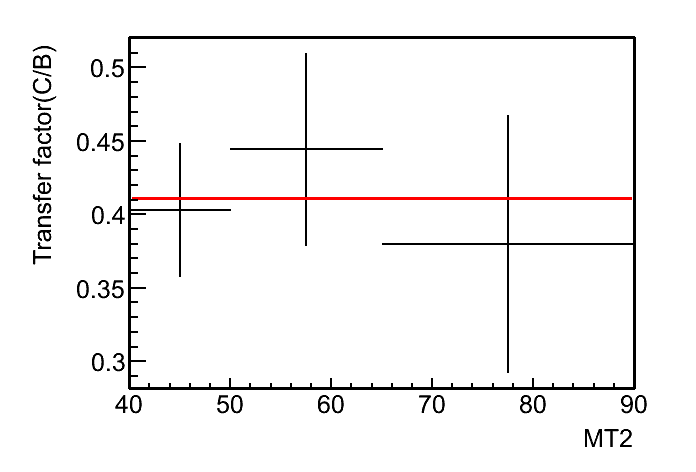
\includegraphics[width=0.49\textwidth]{QCDbginTauTau/Bin1_transferfactor.png}
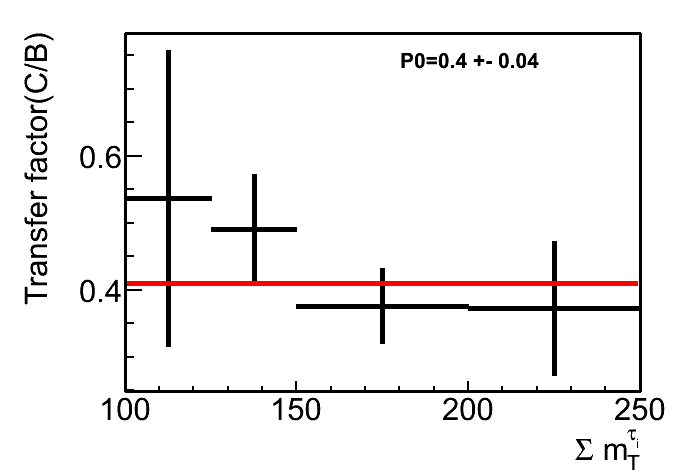
\includegraphics[width=0.49\textwidth]{QCDbginTauTau/Bin2_transferfactor.png} \\
\caption{The ratio of the number of QCD events in the control region C to QCD events in control region B.The
fit line  is drawn in red.
 Left:  $MT2>90$ Bin1   Right:  $\Sigma M_{T}^{\tau} >250$ Bin2.}
\label{fig:1QCDbg}
\end{figure}

The tau identification criterion (tau-id) and a kinematic variable chosen depending (MT2 in Bin 1 and \SumMT in Bin2) 
on the SR are used as the two uncorrelated discriminating variables to define the regions A, B, C and D. The definitions of the control regions are summarized in table \ref{2QCDbg}.

\begin{table}
\begin{center}
\begin{tabular}{|c|c|c|c|}
\hline
Region&A& B & C
\\ \hline\hline
$MT2>90$ Bin1 &$MT2 >90$ & $MT2 <90$&$MT2 <90$ \\
 &at least 1 loose taus&at least 1 loose taus& loose tau veto\\
 &loose-loose loose-medium &loose-loose loose-medium &medium-medium \\
 &loose-tight&loose-tight&medium-tight tight-tight\\ 
 &No cut on charge&No cut on charge& Sum charge==0\\
\hline
$\Sigma M_{T}^{\tau}>250$ Bin2 &$\Sigma M_{T}^{\tau} >250$ &$\Sigma M_{T}^{\tau} <250$&$\Sigma M_{T}^{\tau} < 250$\\
 &at least 1 loose taus&at least 1 loose taus& loose tau veto\\
 &loose-loose loose-medium &loose-loose loose-medium &medium-medium \\
 &loose-tight&loose-tight&medium-tight tight-tight\\
 &No cut on charge&No cut on charge& Sum charge==0\\
% &misc.MinMetJetDphiPt40$>$1 is relaxed\\

\hline
\end{tabular}
\caption{The requirement on the kinematic variables used to define the control regions A,B,C.
MinMetJetDphiPt40$>$1 cut is relaxed. }
\label{2QCDbg}
\end{center}
\end{table}

The number of QCD multi-jet events in the control regions is estimated from data after subtraction of other SM contributions estimated from MC simulation.

In order to increase the data statistics, the cut on the $MinMetJetDphiPt40>1$ is relaxed.This cut was
introduced to suppress the QCD background events,now that we want to estimate QCD multi-jet background this cut is relaxed  .The only the ratio this efficiency should be
applied into account QCD in the control regions to estimate the number of QCD events in the signal region.

The fraction of QCD events with all selection cuts with respect to the QCD events with all selection cuts but the
$MinMetJetDphiPt40>1$ are shown in Figure~\ref{fig:3QCDbg} .

\begin{figure}[htbp]
\centering
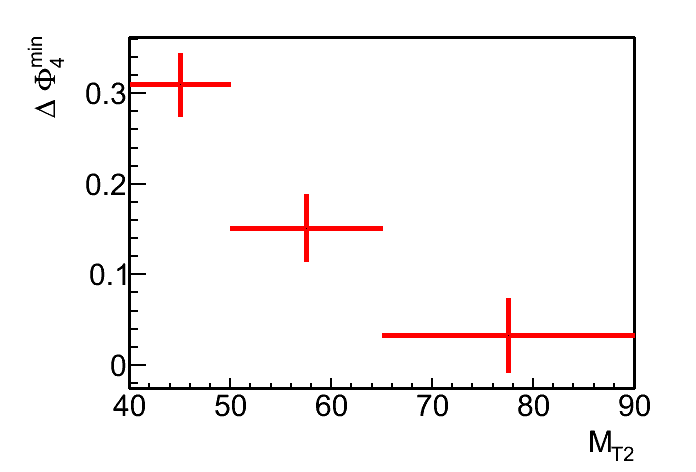
\includegraphics[width=0.49\textwidth]{QCDbginTauTau/Bin1_miscefficiency.png}
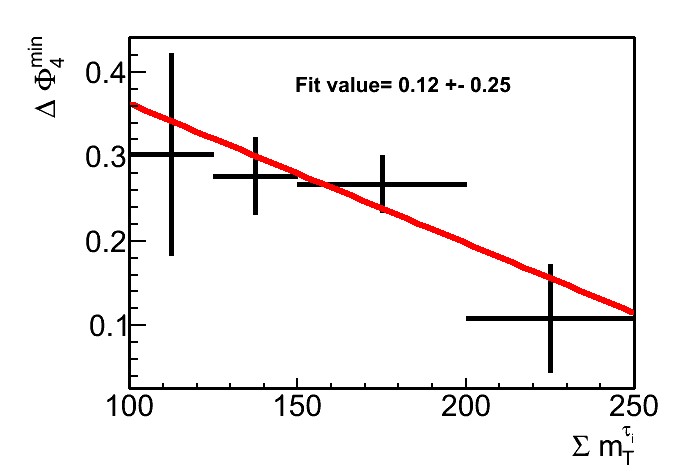
\includegraphics[width=0.49\textwidth]{QCDbginTauTau/Bin2_miscefficiency.png} \\
\caption{ Ratio between QCD multi-jet events passing all selection cuts versus QCD events
 passing all selection cuts but $MinMetJetDphiPt40>1$. Left:  $MT2>90$ Bin1   Right:  $\Sigma M_{T}^{\tau} >250$ Bin2.}
\label{fig:3QCDbg}
\end{figure}




The results of the ABCD method are summarized in table \ref{4QCDbg} and the distributions of the kinematic variables  for data, SM backgrounds and SUSY are shown in the Figure~\ref{fig:5QCDbg}. The SM background distributions
are taken from MC simulation, except for the QCD-multi-jet contribution, which is estimated
using the ABCD method.



\begin{table}
\begin{center}
\scalebox{0.92}{
\begin{tabular}{|l|c|c|c|c|c|c|c|}
\hline
 & Sample & RegionA & RegionB & RegionC & T=C/B & QCD in Signal
 Region(D)\\
\hline\hline
\multirow{7}{*}{MT2$>$90}& Data&10.00 +- 3.16 & 880.00 +- 29.66&  430.00 +- 20.74& \multirow{7}{*}{0.43+-0.32} & \multirow{7}{*}{0.06 +- 0.08}\\ \cline{2-5}

&Z+jets& 2.27 +- 0.90 &29.27 +- 3.22 & 51.45 +- 4.43 & & \\\cline{2-5}

&W+jets& 2.90 +- 1.43&69.20 +- 8.70 &49.25 +- 7.22 & & \\\cline{2-5}

&WW+jets&0.12 +- 0.07 &0.76 +- 0.17 &1.60 +- 0.25 & & \\\cline{2-5}

&Top& 0.49 +- 0.47&21.78 +- 3.13 & 14.51 +- 2.63& & \\\cline{2-5}
&QCD& 4.23 +- 3.62 & 758.99+-31.24& 313.19+-22.55& & \\\cline{2-5}
&Susy& 1.46 +- 0.17& 3.96 +- 0.28& 9.01 +- 0.41& & \\\cline{2-5}
\hline\hline\hline
\multirow{7}{*}{$\Sigma M_{T}^{\tau}>250$}&Data  &25.00 +- 5.00  &723.00 +- 26.89 &348.00 +- 18.65 & \multirow{7}{*}{ 0.41 +- 0.03} & \multirow{7}{*}{0.61 +- 1.55} &  \\
\cline{2-5}


&Z+jets& 2.22 +- 1.07 & 21.78 +- 2.72 & 39.57 +- 3.94& & \\\cline{2-5}

&W+jets&  4.28 +- 1.46&51.84 +- 7.48 & 40.09 +- 6.82& & \\\cline{2-5}

&WW+jets&  0.09 +- 0.05& 0.42 +- 0.13& 0.87 +- 0.19 & & \\\cline{2-5}

&Top&0.42 +- 0.41 &3.07 +- 1.22 & 3.31 +- 1.43& & \\\cline{2-5}
&QCD&18.00 +- 5.33 &645.89+-28.07 & 264.16+-20.30& & \\\cline{2-5}
&Susy& 2.13 +- 0.20&1.18 +- 0.15 &  2.80 +- 0.22& & \\\cline{2-5}
\hline\hline

\end{tabular}}
\caption{ The MC predicted backgrounds in the multi-jet control regions, including both the
statistical and systematic uncertainties, and the expected multi-jet contribution,obtained
by subtracting the MC contributions from observed data . Predicted event yields for the
SUSY  in the control regions are also shown. The estimated multi-jet contribution
in the SRs is given in the last column.
}
\label{4QCDbg}
\end{center}
\end{table}


\begin{figure}[htbp]
\centering
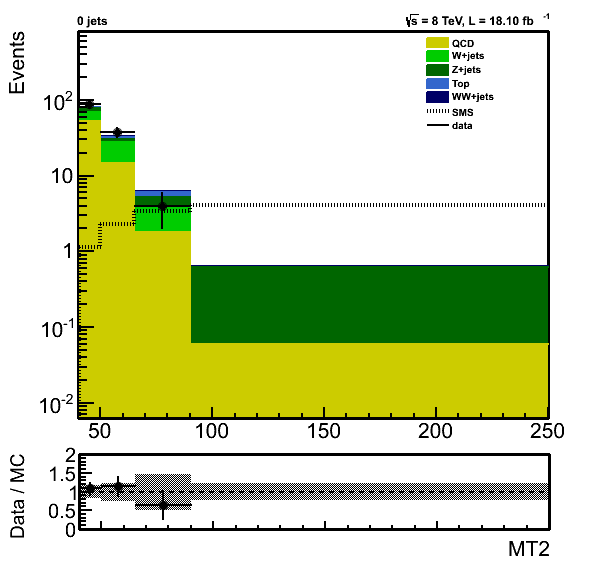
\includegraphics[width=0.49\textwidth]{QCDbginTauTau/Bin1_QCDdatadriven2.png}
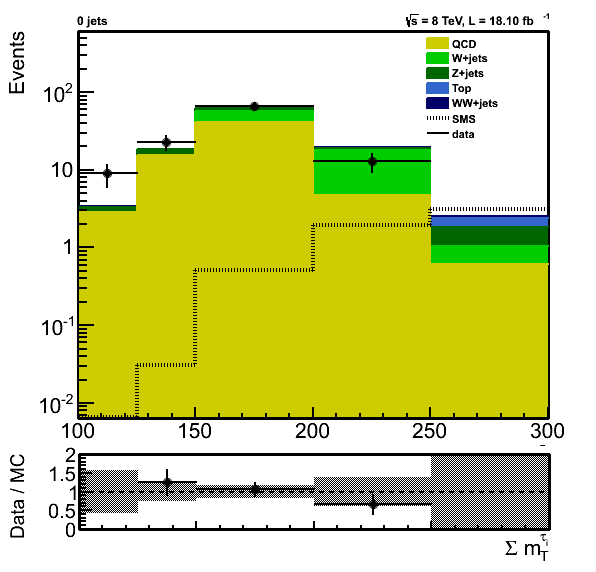
\includegraphics[width=0.49\textwidth]{QCDbginTauTau/Bin2_QCDdatadriven2.png} \\
\caption{Distributions of relevant kinematic variables before the requirement on the given variable
is applied: (a) MT2  (b) $\Sigma M_{T}^{\tau}$ . The QCD multi-jet contribution is estimated from data using the ABCD method.}
\label{fig:5QCDbg}
\end{figure}















 
\section{Systematic uncertainties}
\label{sect:sys}
Systematic uncertainties can affect the shape or normalization of the
backgrounds estimated from Monte Carlo (\ttbar, $Z+$ jets, dibosons and Higgs decays and \wjets in \tauTau \bintwo), 
as well as the signal acceptance.
These uncertainties are listed below and summarized in Table~\ref{Tab.SYS}.
\begin{table}[!h]
\begin{center}
\small{
\begin{tabular}{|l|c|c|c|c|}
\hline\hline
Systematic uncertainty source & \eTau & \muTau & \tauTau SR1 & \tauTau SR2\\
\hline\hline
{Luminosity}&\multicolumn{4}{c|}{$2.6\%$} \\\hline
{$\tau_{had}$ energy scale}&\multicolumn{4}{c|}{$25\%$} \\\hline
{Electron trigger, id, iso efficiency}& $2\%$ & \multicolumn{3}{c|}{} \\\hline
{Muon trigger, id, iso efficiency}& &$2\%$ & \multicolumn{2}{c|}{} \\\hline
{$\tau_{had}$ id efficiency}& \multicolumn{4}{c|}{$6\%$} \\\hline
{$\tau_{had}$ trigger efficiency}& \multicolumn{2}{c|}{$3\%$}&\multicolumn{2}{c|}{$4.5\%$ per leg} \\\hline
{Pile-up}&\multicolumn{4}{c|}{$4\%$} \\\hline
{\MET}&\multicolumn{4}{c|}{$5\%$} \\\hline
{b-jet ID}& $4\%$ & $4\%$ & - & $4\%$ \\\hline
Total(backgrounds) & $26\%$ & $26\%$ & $27\%$  & $27\%$\\\hline
Low rate backgrounds &50\%  & 50\%   & 50\%    & 50\%\\\hline
\multicolumn{5}{|c|}{only for signal} \\\hline
{ISR}&\multicolumn{4}{c|}{$3\%$} \\\hline
{$\mindphifour$}&\multicolumn{4}{c|}{$6\%$} \\\hline
{$\tau_{had}$ energy scale}&\multicolumn{4}{c|}{$15\%$} \\\hline
{PDF}&\multicolumn{4}{c|}{$2\%$} \\\hline
{b-jet ID}& $8\%$ & $8\%$ & - & $8\%$ \\\hline
Total(Signal) & $20\%$ & $20\%$ & $19\%$  & $20\%$\\
\hline
\hline
\end{tabular}
}
\end{center}
\caption{
  Summary of systematic uncertainties.
}
\label{Tab.SYS}
\end{table}


\begin{itemize}

\item The uncertainty on the luminosity  is $2.6\%$.  This affects the
  normalization of all Monte Carlo samples.
 
\item  The systematic uncertainties on the muon and electron energy scales
  are negligible.  In the case of \Tau, the visible energy in the Monte Carlo
  is scaled up and down by $3\%$, and all \Tau-related variables are
  recalculated.  The resulting variations in final yields are taken as
  systematic
  uncertainties.  They amount to 25\% for backgrounds and 15\% for signal.
  In the part of the signal phase space which is accessible by the analysis,
  the value is almost constant in different points and a conservative value is selected.
 % {\bf (Doesn't the signal uncertainty depend on the signal point?)}

\item The uncertainty on electron and muon trigger, identification, and
  isolation efficiencies is $2\%$.
%  {\bf (Shoudn't you say how you obtained these?)}

\item The uncertainty on the $\hadtau$ identification efficiency is $6\%$. 
  The uncertainty on the efficiency of the \Tau leg of the $e\hadtau$ and
  $\mu\hadtau$ ($\tauTau$) triggers amount to $3.0\%$ ($4.5\%$ per leg).
  A ``tag-and-probe'' technique on $\cPZ\to \Pgt\Pgt$ events is used to estimate the 
  uncertainties.
%  {\bf (Shoudn't you say how you obtained these?)}

\item To evaluate the uncertainty due to pileup, the assumed inelastic
  pp cross-section is varied by 5\%.  This then changes the number
  of simulated pileup interactions, and changes the relevant acceptance
  to the processes of interest by $~4 \%$.

\item The uncertainty on the signal acceptance due to parton-distribution
  function uncertainties is expected to be small.
  It is about $2\%$ in the similar analysis \cite{Khachatryan:2014qwa}.
%  {\bf (I am not sure you can get away with thise statement in a paper!)}

\item The uncertanty on the signal acceptance associated with initial state
  radiation (ISR) is evaluated by comparing the efficiency of jet-related
  requirements between \PYTHIA and \MADGRAPH which is a matrix element generator 
  for the $WW$ SM process which
  is similar to chargino pair-production.  From these studies we estimate
  a 3\% uncertainty on the bveto efficiency and a 6\% uncertainty on the
  $\Delta \Phi$ requirement.
  The ISR uncertainty is not considered for the background samples, due to the
  usage of  matrix element  generators.
%  {\bf (This is not correct.  First of all Madgraph is not NLO, it is
%    only partly NLO.  Second, we have a prescription in the SUSY group on how
%    to reweight and/or assign a systematic due to the modeling of
%    the \ttbar transverse momentum)}


%\noindent {\bf What about the btag uncertainty from the btag group?  What about the uncertainty associated with \MET resolution and tails that would throw some of your SM backgrounds like \ttbar or WW into the MT2 tail?  What about the uncertainties on the normalization of the cross-sections for the backgrounds that you take from Monte Carlo?}
\item The \MET uncertainty receives contribution from different sources. The lepton, \Tau, jet energy scale 
(2–10\% depending on $\eta$ and \PT) and unclustered energy scale (10\%). The ``unclustered energy'' stands for the energy of the 
reconstructed objects which do not belong to a jet or lepton with \PT $>$ 10 \GEV.
The effect of lepton and \Tau energy scale are already discussed. The contribution of the jet energy scale and unclustered energy is 
found to be negligible. A conservative relative uncertainty of 5\% is assigned to the signal and background events which are read from the 
Monte Carlo simulation.
\item For some backgrounds like \ttbar,  dibosons and Higgs decays, the remaining 
events from the simulation are very small. A 50\% uncertainty is considered for these backgrounds to account for the theoretical uncertainty of the
cross section calculation as well as the shape mismodeling.
\end{itemize}


\noindent We add all systematic uncertainties in quadrature and assign 
 20\% and 25\% relative uncertainties on the signal
acceptance and the Monte Carlo background predictions, respectively. The relative uncertainty of the 
less important backgrounds is 50\%.



\section[Statistics]{Statistical Interpretation of the results}\label{sect:stat}

\newcommand{\PSGcpmDo}{\ensuremath{\widetilde{\chi}_{1}^{\pm}}\xspace}


Since no excess of data over the background prediction has been observed, 
we close our study with setting upper limits on the testing signals.
This is conducted using a modified frequentist approach, namely CLs method \cite{read:CLs}.
In this method, the test statistic $q_\mu$ \cite{cowan:asymptoticCLs} is a function of the profile likelihood-ratio,

\begin{align}
q_\mu = -2 \ln \frac{\mathcal{L}(data ;\, b + \mu s)}{\mathcal{L}(data ;\, b + \hat{\mu} s)},
\end{align}

where $\hat\mu$ is the \textit{signal strength modifier} $\mu$ at the maximum point of the likelihood $\mathcal{L}$.
Then CLs is given by the following probability-ratio,

\begin{align}
CL_s = \frac{p(q_\mu \geq q_\mu^{obs} | b + \mu s )}{p(q_\mu \geq q_\mu^{obs} | b)}.
\end{align}
 
We compute CLs using a software package provided by the CMS Higgs PAG \cite{higgspag:software}.
After incorporating systematic uncertainties, an observed CLs smaller than 0.05 for a signal strength of $\mu = 1$, excludes the given signal at $95\%$ CL. Indeed, the package determines which signal strength $\mu$ excludes the testing signal at $95\%$ CL. Therefore all resulting $\mu \leq 1$ define the excluded region in the parameter space of the given signal. 


To investigate the exclusion power of our research, we study the topology of direct stau pair production and the $\PSGcpDo\PSGcmDo$ production in Simplified Models \cite{alves:sms}. 
This research deal with tau family decay of charginoes including 
$ \PSGcpmDo \rightarrow \sTau + \nu ~~\mathrm{and}~~  \PSGcpmDo \rightarrow \sNu_{\tau} + \tau $.
As discussed in Section \ref{sect:introduction}, the final state is full of $ \tau $ and $ \sTau \rightarrow \tau + \PSGczDo  $.
Hence many channels could be define, due to decays of tau to electrons, muons and hadrons.    


In this analysis, we examine the data in three different channels.
These channels include $\tau_{had}-\tau_{had}~$, $\mu-\tau_{had}~$ and $e-\tau_{had}~$.
The signal region for the $\mu-\tau_{had}~$ and $e-\tau_{had}~$ channels is defined in one bin, which is $MT2 > 90$ and $tauMT > 200$ .
Due to the sensitivity of $\tau_{had}-\tau_{had}~$ channel to the signal, we look at the data in two different bins.
The first bin is $MT2 > 90$ and the second one is $40 < MT2 < 90$ and $sumMT>250$.
We eventually combine all four bins to utilize more information from the observed and the predicted distributions.
Panels represented in Figure \ref{fig:limit_bins} show the impact of each bin on the combined result, represented by the final exclusion limit shown in Figure \ref{fig:limit_final}. The top-left panel of Figure \ref{fig:limit_bins} shows the expected exclusion region in the plane of $m_{PSGcpmDo}-m_{\PSGczDo}$
calculated by the simulated samples in the first bin of $\tau_{had}-\tau_{had}~$ channel. The top-right panel in Figure \ref{fig:limit_bins} is produced by using both bins of $\tau_{had}-\tau_{had}~$ channel.
As seen, the inclusion of bin 2 in the $\tau_{had}-\tau_{had}~$ channel causes a little expansion of the exclusion limit toward the left side (low mass 
$\PSGcpmDo$).
Two bottom panels of Figure \ref{fig:limit_bins} show the expected exclusion limit when $e-\tau_{had}~$ (left) and $\mu-\tau_{had}~$ (right) channels are included in the $\tau_{had}-\tau_{had}~$ channel.  As seen, each channel individually improves the limit on the right side of plane (high mass $\PSGcpmDo$).


%%%%%%%%%%
\begin{linenomath}
\begin{figure}[h]
\centering
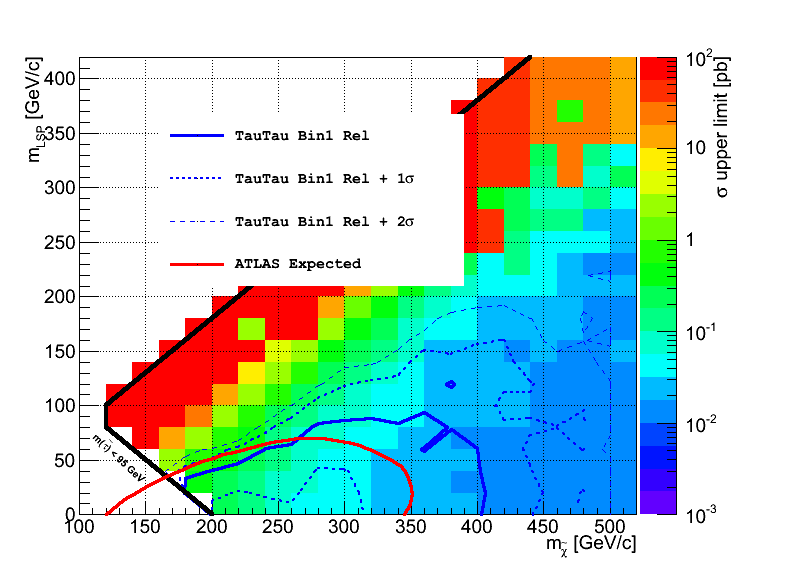
\includegraphics[width=0.49\textwidth,keepaspectratio=true]{StatisticsFig/NewFigs/TauTau_Bin1Rel.png}
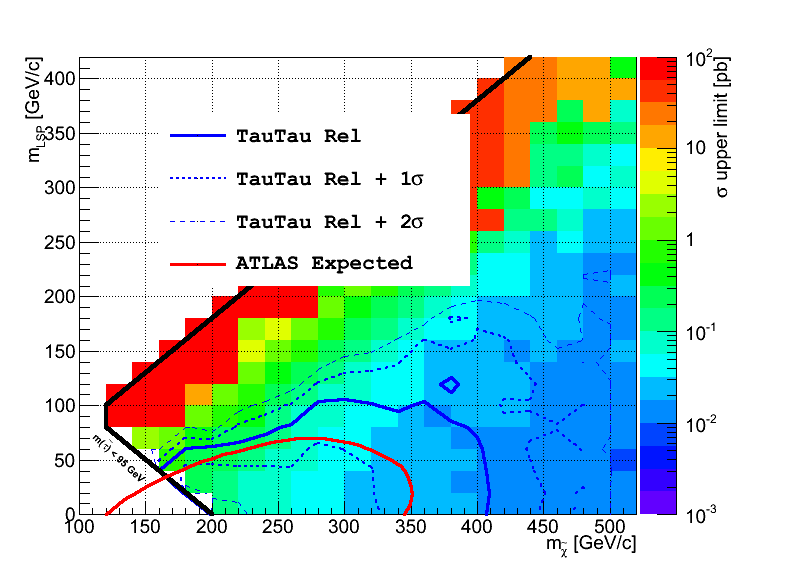
\includegraphics[width=0.49\textwidth,keepaspectratio=true]{StatisticsFig/NewFigs/TauTau_Bin1Rel_Bin2.png}
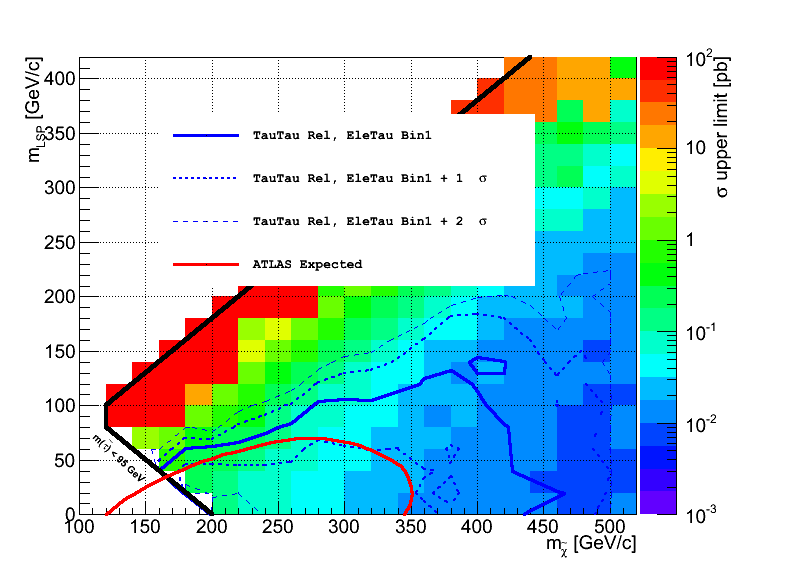
\includegraphics[width=0.49\textwidth,keepaspectratio=true]{StatisticsFig/NewFigs/TauTau_EleTauBin1.png}
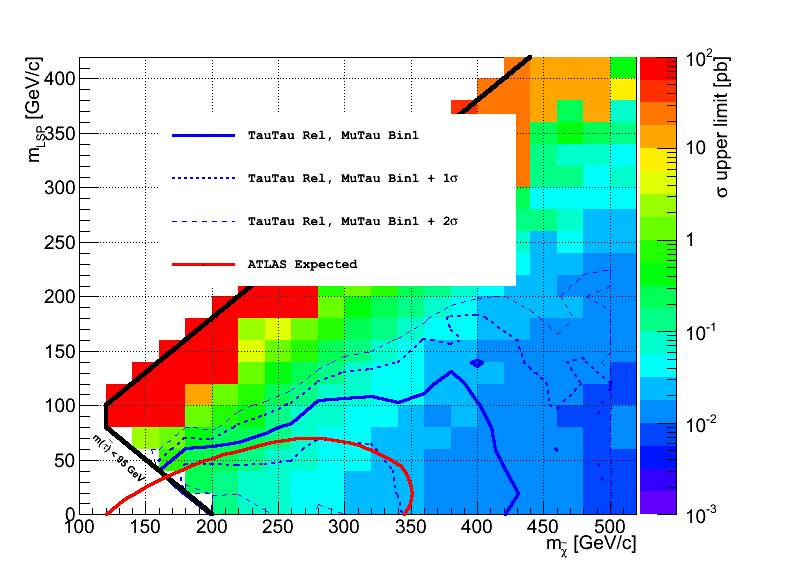
\includegraphics[width=0.49\textwidth,keepaspectratio=true]{StatisticsFig/NewFigs/TauTau_MuTauBin1.png}
\caption{These figures show the impact of each bin on the final combination. 
The top panels are related to the $\tau_{had}-\tau_{had}~$ channel including the bin 1 alone (left) and combination of bins 1 and 2 (right).
The bottom ones show the expected exclusion limit when $e-\tau_{had}~$ (left) and $\mu-\tau_{had}~$ (right) channels are included in the $\tau_{had}-\tau_{had}~$ channel.
}
\label{fig:limit_bins}
\end{figure}
\end{linenomath}
%%%%%%%%%%


Figure \ref{fig:limit_final} shows the expected upper limit on the cross section of the chargino pair production in terms of Simplified Models. 
The signal rates for each bin are 0.5420, 1.7200, 1.5800 and 0.7680, 
while overall background rates are 3.01, 1.5, 2.7 and 1.06 respectively.
However, backgrounds are taken into account in two categories, including Monte-Carlo-Driven (MCD), Data-Driven (DD).
Due to the method of background estimation in the $\tau_{had}-\tau_{had}~$ channel, bins 1 and 2 have a more category called W-jets (W).    
MCD backgrounds are feed to the package as a Gamma distribution with the corresponding statistical weights for each bin.
Furthermore, 25\% systematic uncertainity on MCD backgrounds is also considered.
All systematics are taken through LogNormal distributions.
Systematic uncertainities for each bin of DD backgrounds are 15\%, 11\%, 50\% and 69\% respectively. (numbers must be corrected)  
W backgronds have 37\% and 45\% systematic uncertainity for the first and second bins respectively.
And finally, 20\% systematic uncertainity on signal yields is considered. 
Calculation of the expected exclusion limit shows that the research has potential to exclude 
%excludes 
a sizable region of the phase space, surrounded by the lines of $m_{\PSGcpmDo} = 500\GeV$ and $m_{\PSGczDo} = 150\GeV$ with an integrated luminosity of $19.6\,\fbinv$.
The Red curve represents the expected reach by ATLAS %\cite{cutandcountAN}
 search. As the figure shows our analysis (the blue solid curve) improves the ATLAS result in the $m_{\PSGcpmDo}-m_{\PSGczDo}$ plane.

%%%%%%%%%%
\begin{linenomath}
\begin{figure}[h]
\centering
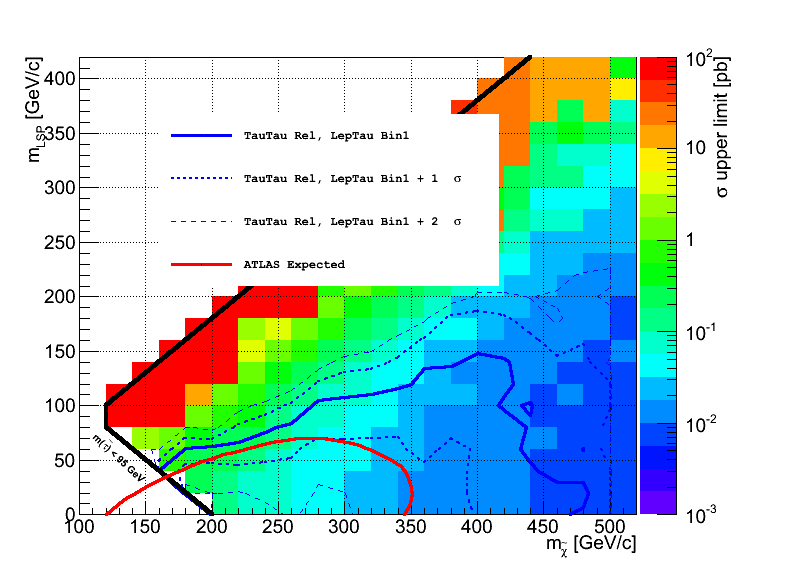
\includegraphics[width=0.7\textwidth,keepaspectratio=true]{StatisticsFig/NewFigs/Final_4BinRel.png}
\caption{Expected exclusion power in terms of Simplified Models %(T2tt-topology) 
with an integrated luminosity of $20\,\fbinv$. Backgrounds are predicted using Monte-Carlo simulations and a rough estimate of systematic uncertainties equal 
$10\%$ is taken into account.}
\label{fig:limit_final}
\end{figure}
\end{linenomath}
%%%%%%%%%%


%\rule{\textwidth}{1pt}

%In this study, we analyze data in 8 different bins (multi-bin analysis) to utilize more information from 
%the observed and the predicted distributions.
%bins' contents of the observations and the predictions.
%The bins are defined in reconstructed top quark multiplicity, zero or more. In addition, events are categorized based on the $\mttwo$ values: $125\GeV \leq \mttwo < 150\GeV,\; 150\GeV \leq \mttwo < 200\GeV,\; 200\GeV \leq \mttwo < 250\GeV,\; 250\GeV \leq \mttwo < \infty$.
%These bins are determined, for an event, based on whether the event contents reconstructed top quarks or not (2 bins) times which bin of $\mttwo$ is occupied by the event (4 bins of $125\GeV \leq \mttwo < 150\GeV,\; 150\GeV \leq \mttwo < 200\GeV,\; 200\GeV \leq \mttwo < 250\GeV,\; 250\GeV \leq \mttwo < \infty$). 

%To investigate the exclusion power of our research, we study the topology of direct stop pair production  in Simplified Models \cite{alves:sms}, with $\tilde{t}\to \PSGczDo t$ (T2tt). 
%Calculation of the expected exclusion limit shows that  
%the research has potential to exclude 
%excludes 
%a sizable region of the phase space, surrounded by the lines of $m_{\tilde{t}} = 600\GeV$ and $m_{\PSGczDo} = 175\GeV$ with an integrated luminosity of $19.6\,\fbinv$.



%Figure \ref{fig:limit_20inf} shows the expected upper limit on the cross section of the stop pair production in terms of Simplified Models. 
%Furthermore, the figure shows the expected exclusion power considering 
%$40\%$ systematic uncertainties on signal and background rates which are predicted using Monte-Carlo simulations. The black 
%dashed curve represents the expected reach by the common Cut$\&$Count \cite{cutandcountAN} search using $\MET$ trigger. 
%As the figure shows our analysis (the blue solid curve) can be comparable with other analyses and   
%it has the potential to be complementary to other analyses in some regions of the phase space.  



%%%%%%%%%%
%\begin{linenomath}
%\begin{figure}[h]
%\centering
%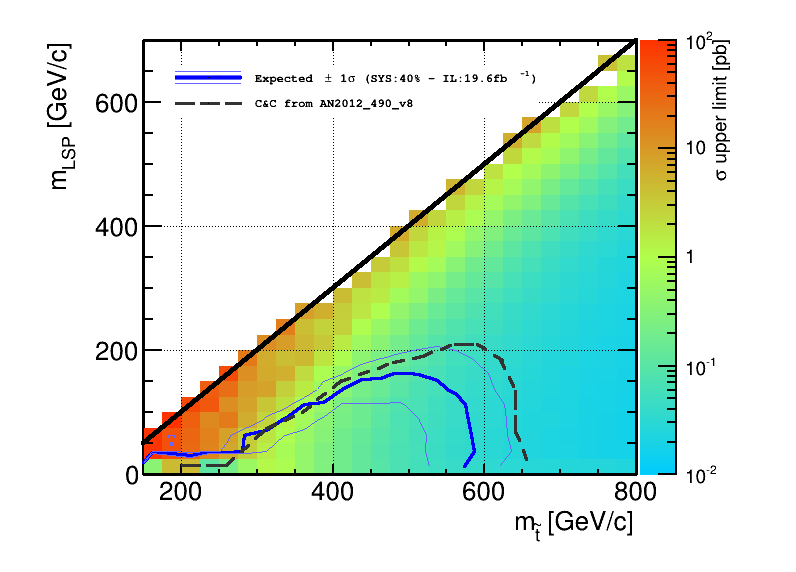
\includegraphics[width=0.9\textwidth,keepaspectratio=true]{StatisticsFig/Exc_131030_196ifb.png}
%\caption{Expected exclusion power in terms of Simplified Models (T2tt-topology) with an integrated luminosity of $20\,\fbinv$. Backgrounds are predicted using Monte-Carlo simulations and a rough estimate of systematic uncertainties equal 
%$40\%$ is taken into account.}
%\label{fig:limit_20inf}
%\end{figure}
%\end{linenomath}
%%%%%%%%%%


%%%%%%%%%%
%\begin{linenomath}
%\begin{figure}[h]
%\centering
%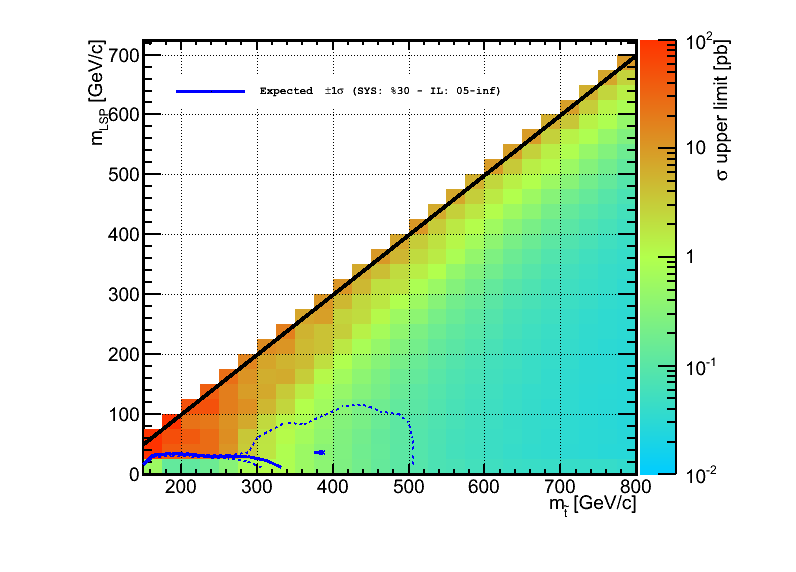
\includegraphics[width=0.7\textwidth,keepaspectratio=true]{StatisticsFig/limit_30sys_05inf_20130625.png}
%\caption{}
%\label{fig:limit_05inf}
%\end{figure}
%\end{linenomath}
%%%%%%%%%%

%%%%%%%%%%
%\begin{linenomath}
%\begin{figure}[h]
%\centering
%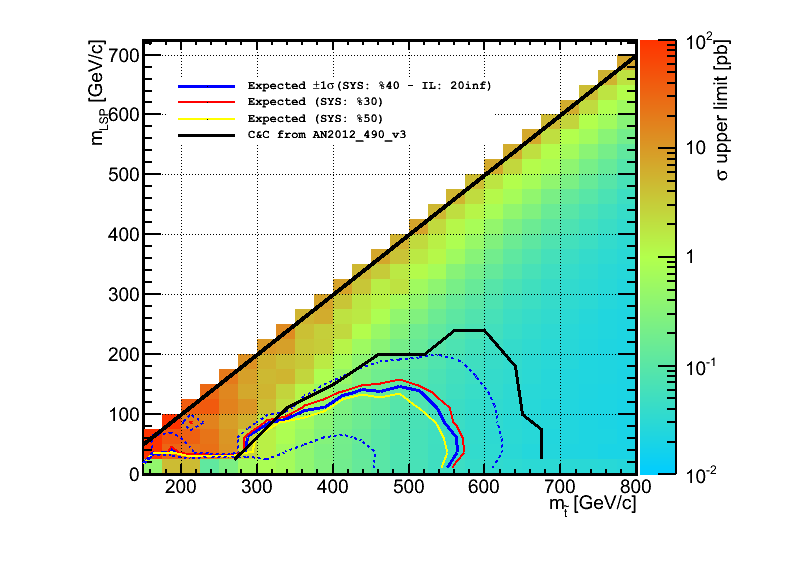
\includegraphics[width=0.7\textwidth,keepaspectratio=true]{StatisticsFig/limit_304050sys_20inf_20130625.png}
%\caption{}
%\label{fig:limit_20inf}
%\end{figure}
%\end{linenomath}
%%%%%%%%%%


\section{Conclusion}
\label{sect:conclusion}
A search for SUSY in $\tau\tau$ final state is presented. The $\tau$ pair is produced in a cascade from the production of the \PSGcpDo pair.
Different channels and search bins are introduced to increase the sensitivity to different parts of the phase space. 
Backgrounds and their systematics are discussed in details. The expected exclusion limits are also presented for different combination of the 
channels.

\section{Acknowledgments}
This analysis benefits highly from the computing resources of T2 at UCSD and codes developed in ETHZurich. 
We appreciate their help and generosity.
The authors would like to thank the previous and current conveners of the SUSY and SUSY-TBT working group, Frank Wuerthwein, Keith Ulmer, Filip Moortgat, Joshua Thompson, Pieter Everaerts and Boris Mangano for their help and support. 
The authors would like to thank the management and staff of the school of particles 
and accelerators of IPM, especially Prof. Arfaei for their help and support. 
We had several discussions with our colleagues at LIP, Pedram Bargassa, Michele Gallinaro and Cristovao Beirao Da Cruz E Silva. 
We would like to thank them for their helps and suggestions.
Thanks to all of the members of
the CMS collaboration for their outstanding results discussed partly here.


\bibliography{auto_generated}
%%% DO NOT ADD \end{document}!
